\clearpage
\phantomsection

\setcounter{chapter}{1}
\chapter[{ĐẶC TẢ KỸ THUẬT}]{Đặc tả kỹ thuật}

%\section{Đặc tả kỹ thuật}
Chương này sẽ cung cấp các thông tin về các yêu cầu chức năng và phi chức năng của IP cần thiết kế, từ mô-đun lớn nhất đến các mô-đun nhỏ hơn. Các thông tin về đặc tả kỹ thuật của IP sẽ bao gồm thông tin về chức năng, danh sách tham số và tín hiệu của mô-đun, kiến trúc ở mức hành vi và mô tả dạng sóng của mô-đun.

\section{Yêu cầu hệ thống }
Bảng \ref{tab:non_functional} đây mô tả các yêu cầu hệ thống cho IP (bao gồm yêu cầu chức năng và yêu cầu phi chức năng):
\begin{table}[!ht]
    \centering
    \renewcommand{\arraystretch}{1.3} % Tăng khoảng cách dòng
        \caption{Các yêu cầu phi chức năng cho thiết kế}
    \begin{tabular}{p{5cm} p{10cm} }
        \toprule
        \textbf{Yêu cầu} & \textbf{Mô tả} \\
        \midrule
        Chức năng & Thực hiện trích xuất đặc trưng sử dụng thuật toán MRELBP
        \\ \midrule
        Thông số kỹ thuật & 
        \begin{tabular}[t]{@{}l@{}}
Các thông số thuật toán: r = 2, 4, 6; p = 8 \\
Độ rộng dữ liệu: Đầu vào 8-bit, đầu ra 32-bit \\
Kích thước ảnh đầu vào: có thể tùy chỉnh theo tham số cấu hình \\
Số lượng dữ liệu đầu ra: 600 dữ liệu \\
Độ chính xác: dấu phẩy tĩnh (16-bit thập phân, 8-bit phần nguyên)
\end{tabular} 
\\
        
        \midrule
        Hiệu suất (Performance) & Tần số hoạt động tối thiểu 100 MHz
        \\ \midrule
        Tính đồng bộ & Tất cả các tín hiệu đồng bộ theo 1 clock chính
        \\ \midrule
        Reset & Tất cả các mô-đun tuân theo reset đồng bộ
        \\ \midrule
        Tài nguyên sử dụng & Tối đa 30000 LUTs, 30000 Registers, 200 DSPs, 100 BRAM 
        \\ \midrule
        Khả năng kiểm thử & Hỗ trợ kiểm thử test-bench ngẫu nhiên và test-bench trực tiếp
        \\ \midrule
        Chuẩn giap tiếp & Có thể tương thích với chuẩn AXI4-Stream
        \\ \midrule
        Tương thích công cụ & Có thể tổng hợp trên các phần mềm như Vivado, Quartus, ...
        \\ \midrule
        Khả năng tích hợp & Có thể giao tiếp IP đối với các IP khác như DMA, ...
        \\ \midrule
        Độ bao phủ & Tối thiểu 80\% về mặt chức năng
        \\ \midrule
        Kiểm thử tự động & Xây dựng hệ thống giúp kiểm thử về mặt chức năng một cách tự động
        \\
        
                        \bottomrule

    \end{tabular}

    \label{tab:non_functional}
\end{table}
\section{Xác định thiết kế}
\subsection{Tối ưu thuật toán phù hợp với phần cứng}
Đồ án sẽ xây dựng IP trích xuất đặc trưng sử dụng thuật toán Median Robust Extended Local Bianry Pattern. Đây là một thuật toán hoạt động tương đối phức tạp với 3 loại đặc trưng được tính toán theo các công thức \ref{eq:relbp_ci}, \ref{eq:relbp_ni}, \ref{eq:relbp_rd}. Tuy nhiên, đối với công thức \ref{eq:relbp_ci}, việc phải lưu lại toàn bộ bức ảnh để tính trung bình sẽ gây ảnh hưởng lớn về mặt thời gian và lưu trữ, do đó, để cải tiến, ta sẽ có mô tả như sau:
    \begin{equation}
        RELBP\_CI(x_c) = s(\phi(\mathbf{X}_{c, w}) - \mu_w)
         \label{eq:relbp_ci_op}
    \end{equation}
    $\begin{cases}
    \phi(\mathbf{X}_{c,w}) \text{ là kết quả sau khi áp dụng bộ lọc lên điểm ảnh } X, \\
    \text{Vùng cục bộ có kích thước } w \times w \text{ ở xung quanh vị trí điểm ảnh trung tâm}, \\
    \mu_w \text{ kí hiệu cho giá trị trung bình của } \phi(X_{c,w}) \text{ trong một vùng cục bộ kích thước w x w}.
\end{cases}$

\begin{figure} [!hht]
	\centering
	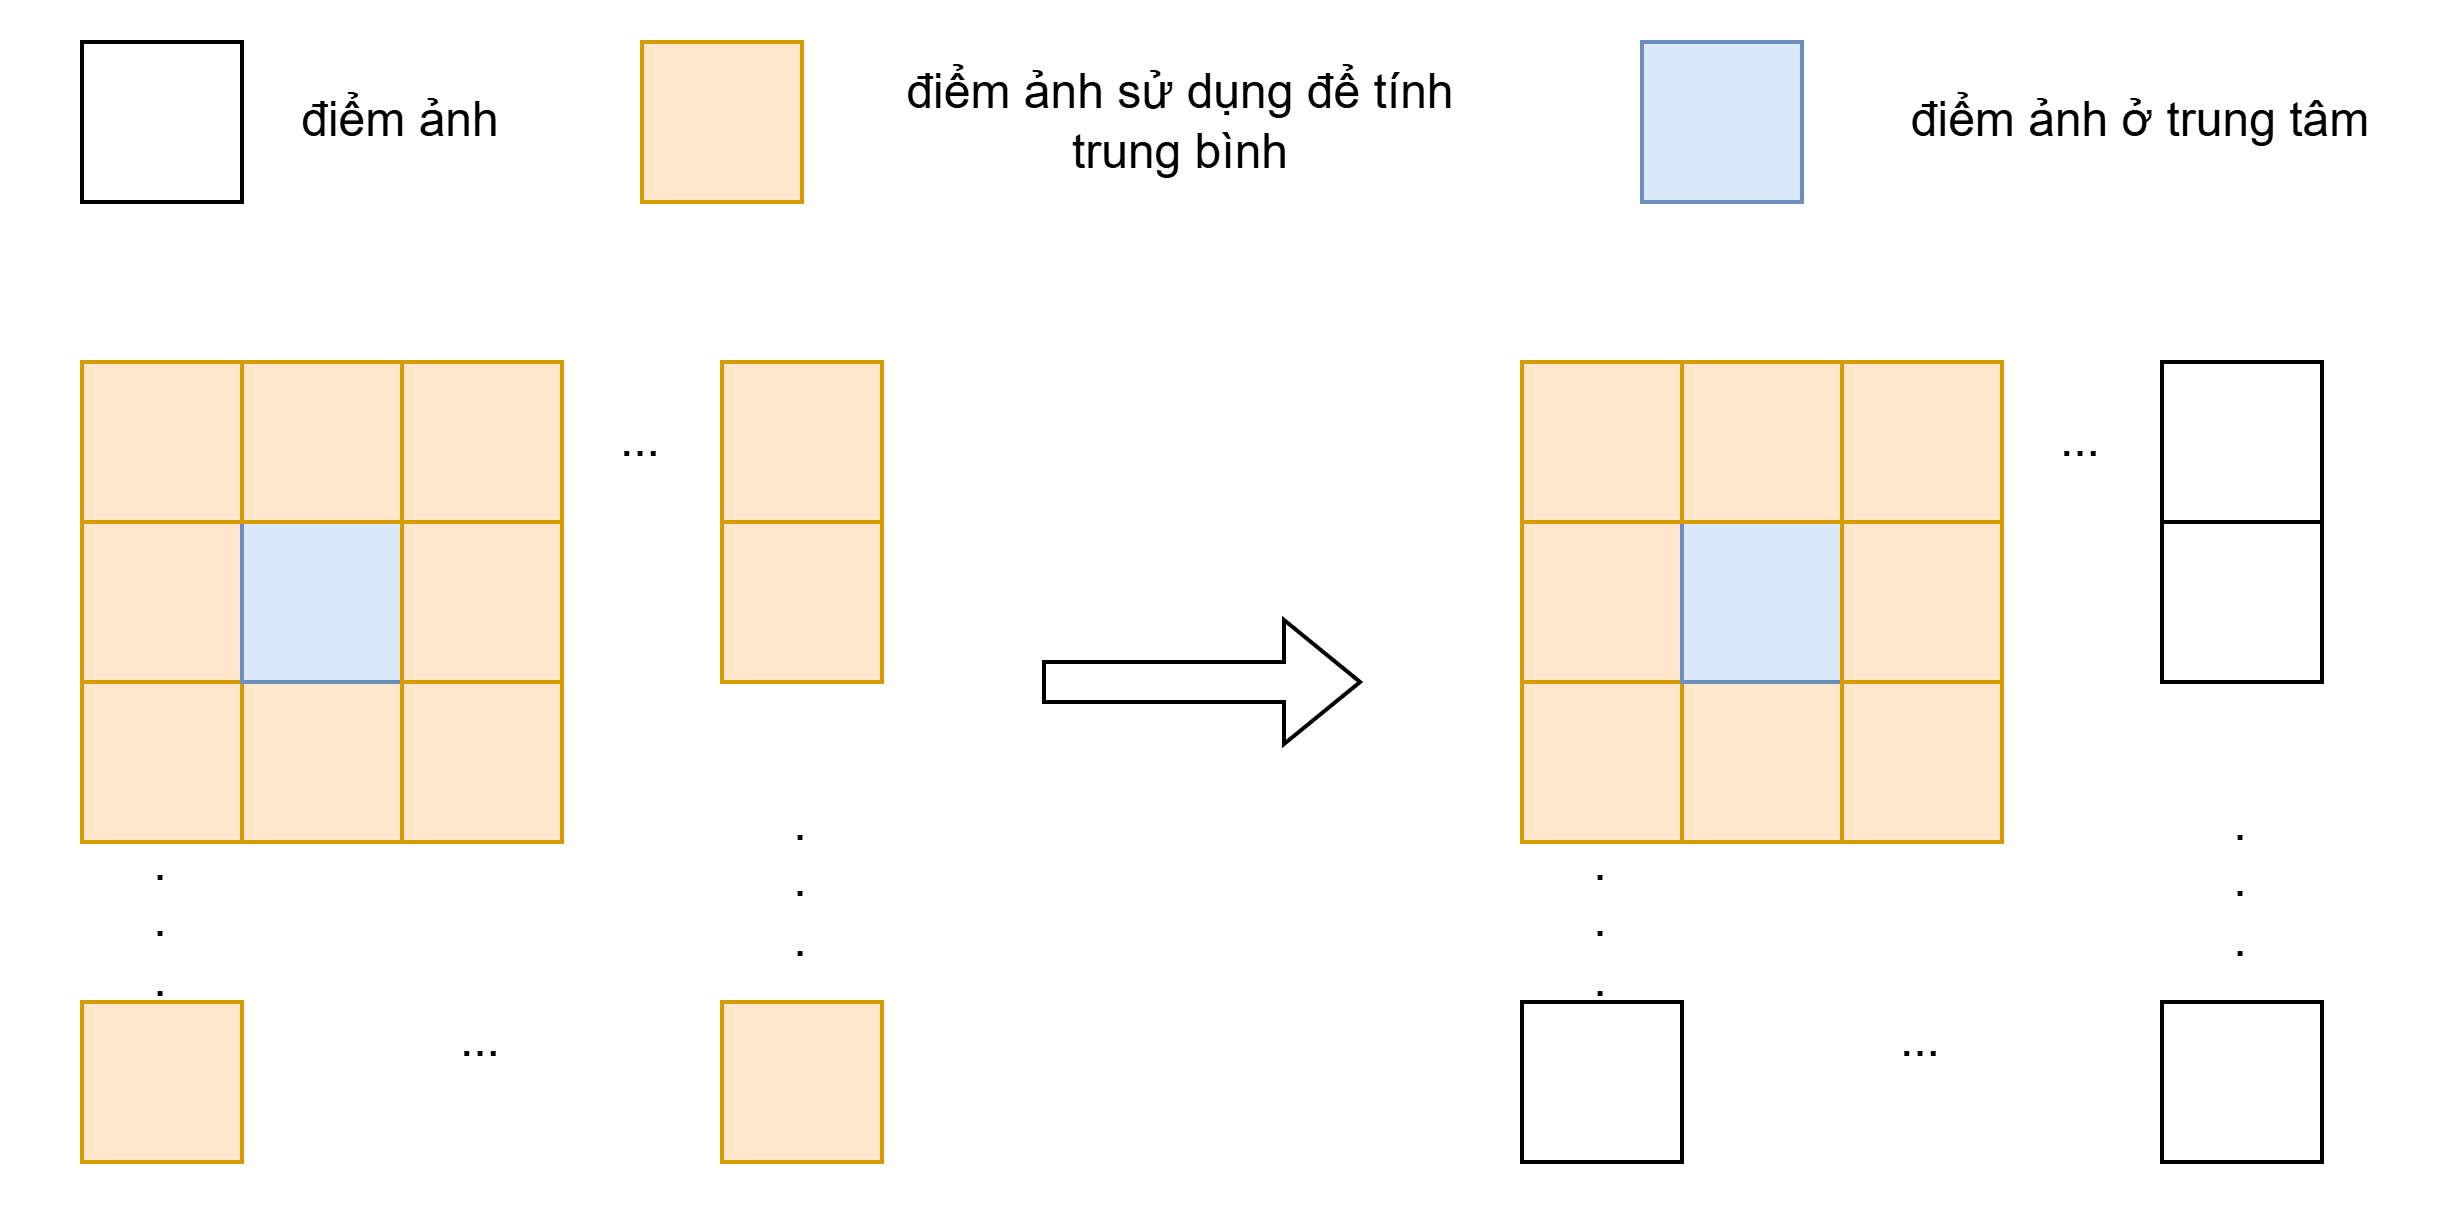
\includegraphics[width=\linewidth]{figures/ciOptimize.png}
	\caption{Phiên bản thiết kế phần cứng của biểu diễn điểm ảnh trung tâm - CI}
	\label{fig:ciOptimize}
\end{figure} 
Hình \ref{fig:ciOptimize} mô tả phiên bản phù hợp hơn của biểu diễn điểm ảnh trung tâm (CI) với việc thay đổi từ tính toán trung bình của toàn bộ bức ảnh thành tính toán trung bình của một vùng nội bộ trong bức ảnh. Điều này sẽ làm tăng tính xử lý thời gian thực của thiết kế lên vì không cần phải lưu lại toàn bộ bức ảnh. Kết quả nghiên cứu của Wang và Zhang \cite{realTimeTexture} đã cho thấy sự thay đổi về tính toán không gây ra sai số quá lớn về độ chính xác, giữ nguyên với Outex\_TC10 với, giảm 0.052\% với tập Outex\_TC12\_000 và giảm 0.104\% với tập Outex\_TC12\_002.

\subsection{Sơ đồ triển khai thuật toán}
Quá trình tạo ra biểu đồ histogram được mô tả theo hình \ref{fig:histogramStep}. Với đầu vào là ảnh kết cấu, sau quá trình lấy mẫu theo các công thức \ref{eq:relbp_ci_op}, \ref{eq:relbp_ni}, \ref{eq:relbp_rd} ta được các mô tả thô của ảnh. Sau đó, thực hiện một giai đoạn là "Joint Histogram", tại giai đoạn này, thực tế ta sẽ đếm xem là mô tả đấy xuất hiện bao nhiêu lần, do đó kết quả đạt được là một biểu đồ histogram. Sau đó ta sẽ nối lần lượt các biểu đồ này lại để được đặc trưng cuối cùng. 

\begin{figure} [!ht]
	\centering
	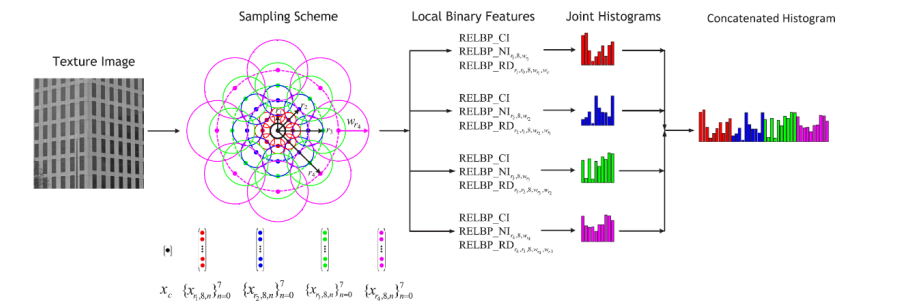
\includegraphics[width= 1\linewidth]{figures/histogramStep.png}
	\caption{Quá trình tạo ra đặc trưng của thuật toán RELBP \cite{realTimeTexture}}
	\label{fig:histogramStep}
\end{figure} 


\begin{figure} [!ht]
	\centering
	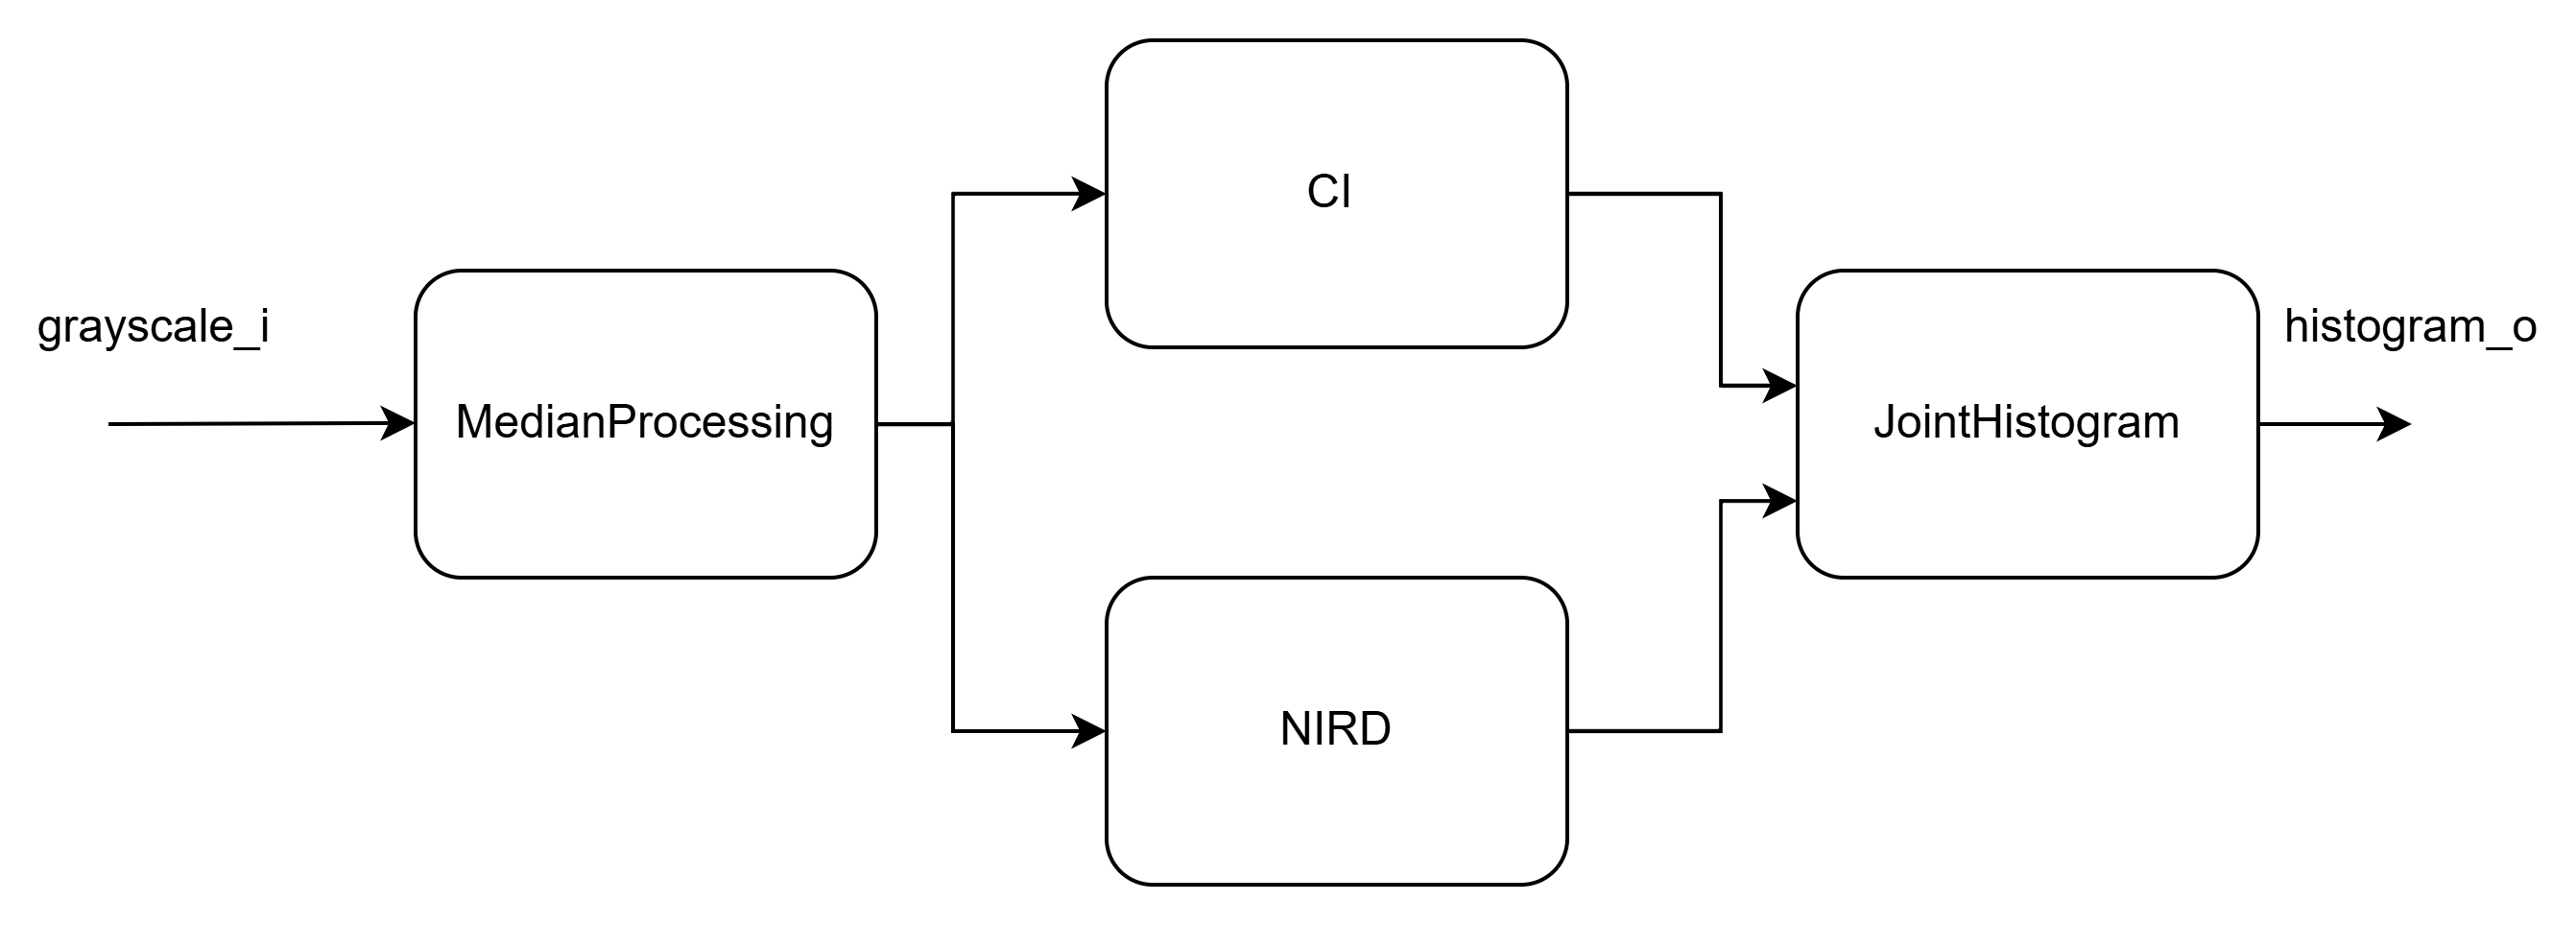
\includegraphics[width= 1\linewidth]{figures/fullArch.png}
	\caption{Sơ đồ kiến trúc tổng quát của MRELBP IP}
	\label{fig:fullArch}
\end{figure} 


Với những mô tả trên, sơ đồ thuật toán được đưa ra như hình \ref{fig:fullArch}. Một cách cụ thể hơn, vì MRELBP là phiển bản của RELBP với $\phi()$ là bộ tính trung vị, nên khi thiết kế phần cứng, ta sẽ đưa ra toàn bộ các phiên bản tính trung vị của ảnh đầu vào. Sau đó, sẽ có 2 bộ là CI và NIRD để tính các giá trị đặc trưng theo mô tả công thức \ref{eq:relbp_ci_op}, \ref{eq:relbp_ni}, \ref{eq:relbp_rd}. Vì NIRD có cách tính và yêu cầu đầu vào tương đối giống nhau, do đó, 2 mô tả này có thể xây dựng trong cùng 1 mô-đun để tiết kiệm tài nguyên. Sau đó 3 mô tả này sẽ thực hiện qua bước "JointHistogram" để đạt được đặc trưng đầu ra.


\section{ Đặc tả kỹ thuật}



\subsection{Đặc tả mô-đun MRELBP}

Bảng \ref{tab:paramListMRELBP}, \ref{tab:signalListMRELBP} mô tả các tham số và tín hiệu đầu vào, đầu ra của mô-đun MRELBP. 
\begin{table}[h]
    \centering
    \renewcommand{\arraystretch}{1.3} % Tăng khoảng cách dòng
        \caption{Danh sách các tham số của mô-đun MRELBP }
    \begin{tabular}{|p{3cm} p{4cm} p{8cm}|}
        \hline
        \rowcolor{gray!30}
        \textbf{Tham số } & \textbf{Giá trị mặc định}  & \textbf{Mô tả} \\
        \hline
        ROWS & 128 & Kích thước chiều cao của ảnh
        \\ \hline
        COLS & 128 & Kích thước chiều rộng của ảnh
        \\ \hline
    \end{tabular}

    \label{tab:paramListMRELBP}
\end{table}

\begin{table}[h]
    \centering
    \renewcommand{\arraystretch}{1.3} % Tăng khoảng cách dòng
        \caption{Danh sách các tín hiệu của giao diện mô-đun MRELBP}
    \begin{tabular}{|p{3cm} p{2cm} p{2cm} p{8cm}|}
        \hline
        \rowcolor{gray!30}
        \textbf{Tên tín hiệu} & \textbf{Độ rộng} & \textbf{Vào ra} & \textbf{Mô tả} \\
        \hline
        clk & 1 & Vào & Tín hiệu clock \\
        \hline
        rst\_n & 1 & Vào & Reset đồng bộ, kích hoạt mức thấp \\
        \hline
        start\_i & 1 & Vào & Tín hiệu bắt đầu (liên quan đến đầu ra)
        \\ \hline
        grayscale\_i & 8 & Vào & Dữ liệu điểm ảnh 
        \\ \hline
        i\_valid & 1 & Vào & Tín hiệu báo hiệu dữ liệu đầu vào là hợp lệ
        \\ \hline
        o\_data\_ready & 1 & Ra & Tín hiệu thông báo sẵn sàng cho đầu ra
        \\ \hline
        histogram\_o & 32 & Ra & Đặc trưng histogram
        \\ \hline
        o\_valid & 1 & Ra & Tín hiệu báo hiệu dữ liệu đầu ra là hợp lệ
        \\ \hline
        i\_data\_ready & 1 & Vào & Tín hiệu thông báo sẵn sàng nhận dữ liệu
        \\ \hline
        o\_intr & 1 & Ra &Tín hiệu báo hiệu đã xử lý xong
        \\ \hline
    \end{tabular}

    \label{tab:signalListMRELBP}
\end{table}


Hình \ref{fig:mrelbpArchitecture} mô tả sơ đồ khối của mô-đun MRELBP một cách chi tiết hơn. mô-đun \textbf{MedianProcessing} được cấu thành từ mô-đun Buffer6Rows, mô-đun ZeroPadding và mô-đun MedianCalculation. Dữ liệu đầu ra là giá trị trung vị của ảnh, sau đó sẽ đi đến các mô-đun sau là \textbf{CI} và \textbf{NIRD}. Mô tả chi tiết hơn về đường đi của dữ liệu sẽ được giới thiệu tại các phần sau.
\begin{figure} [!ht]
	\centering
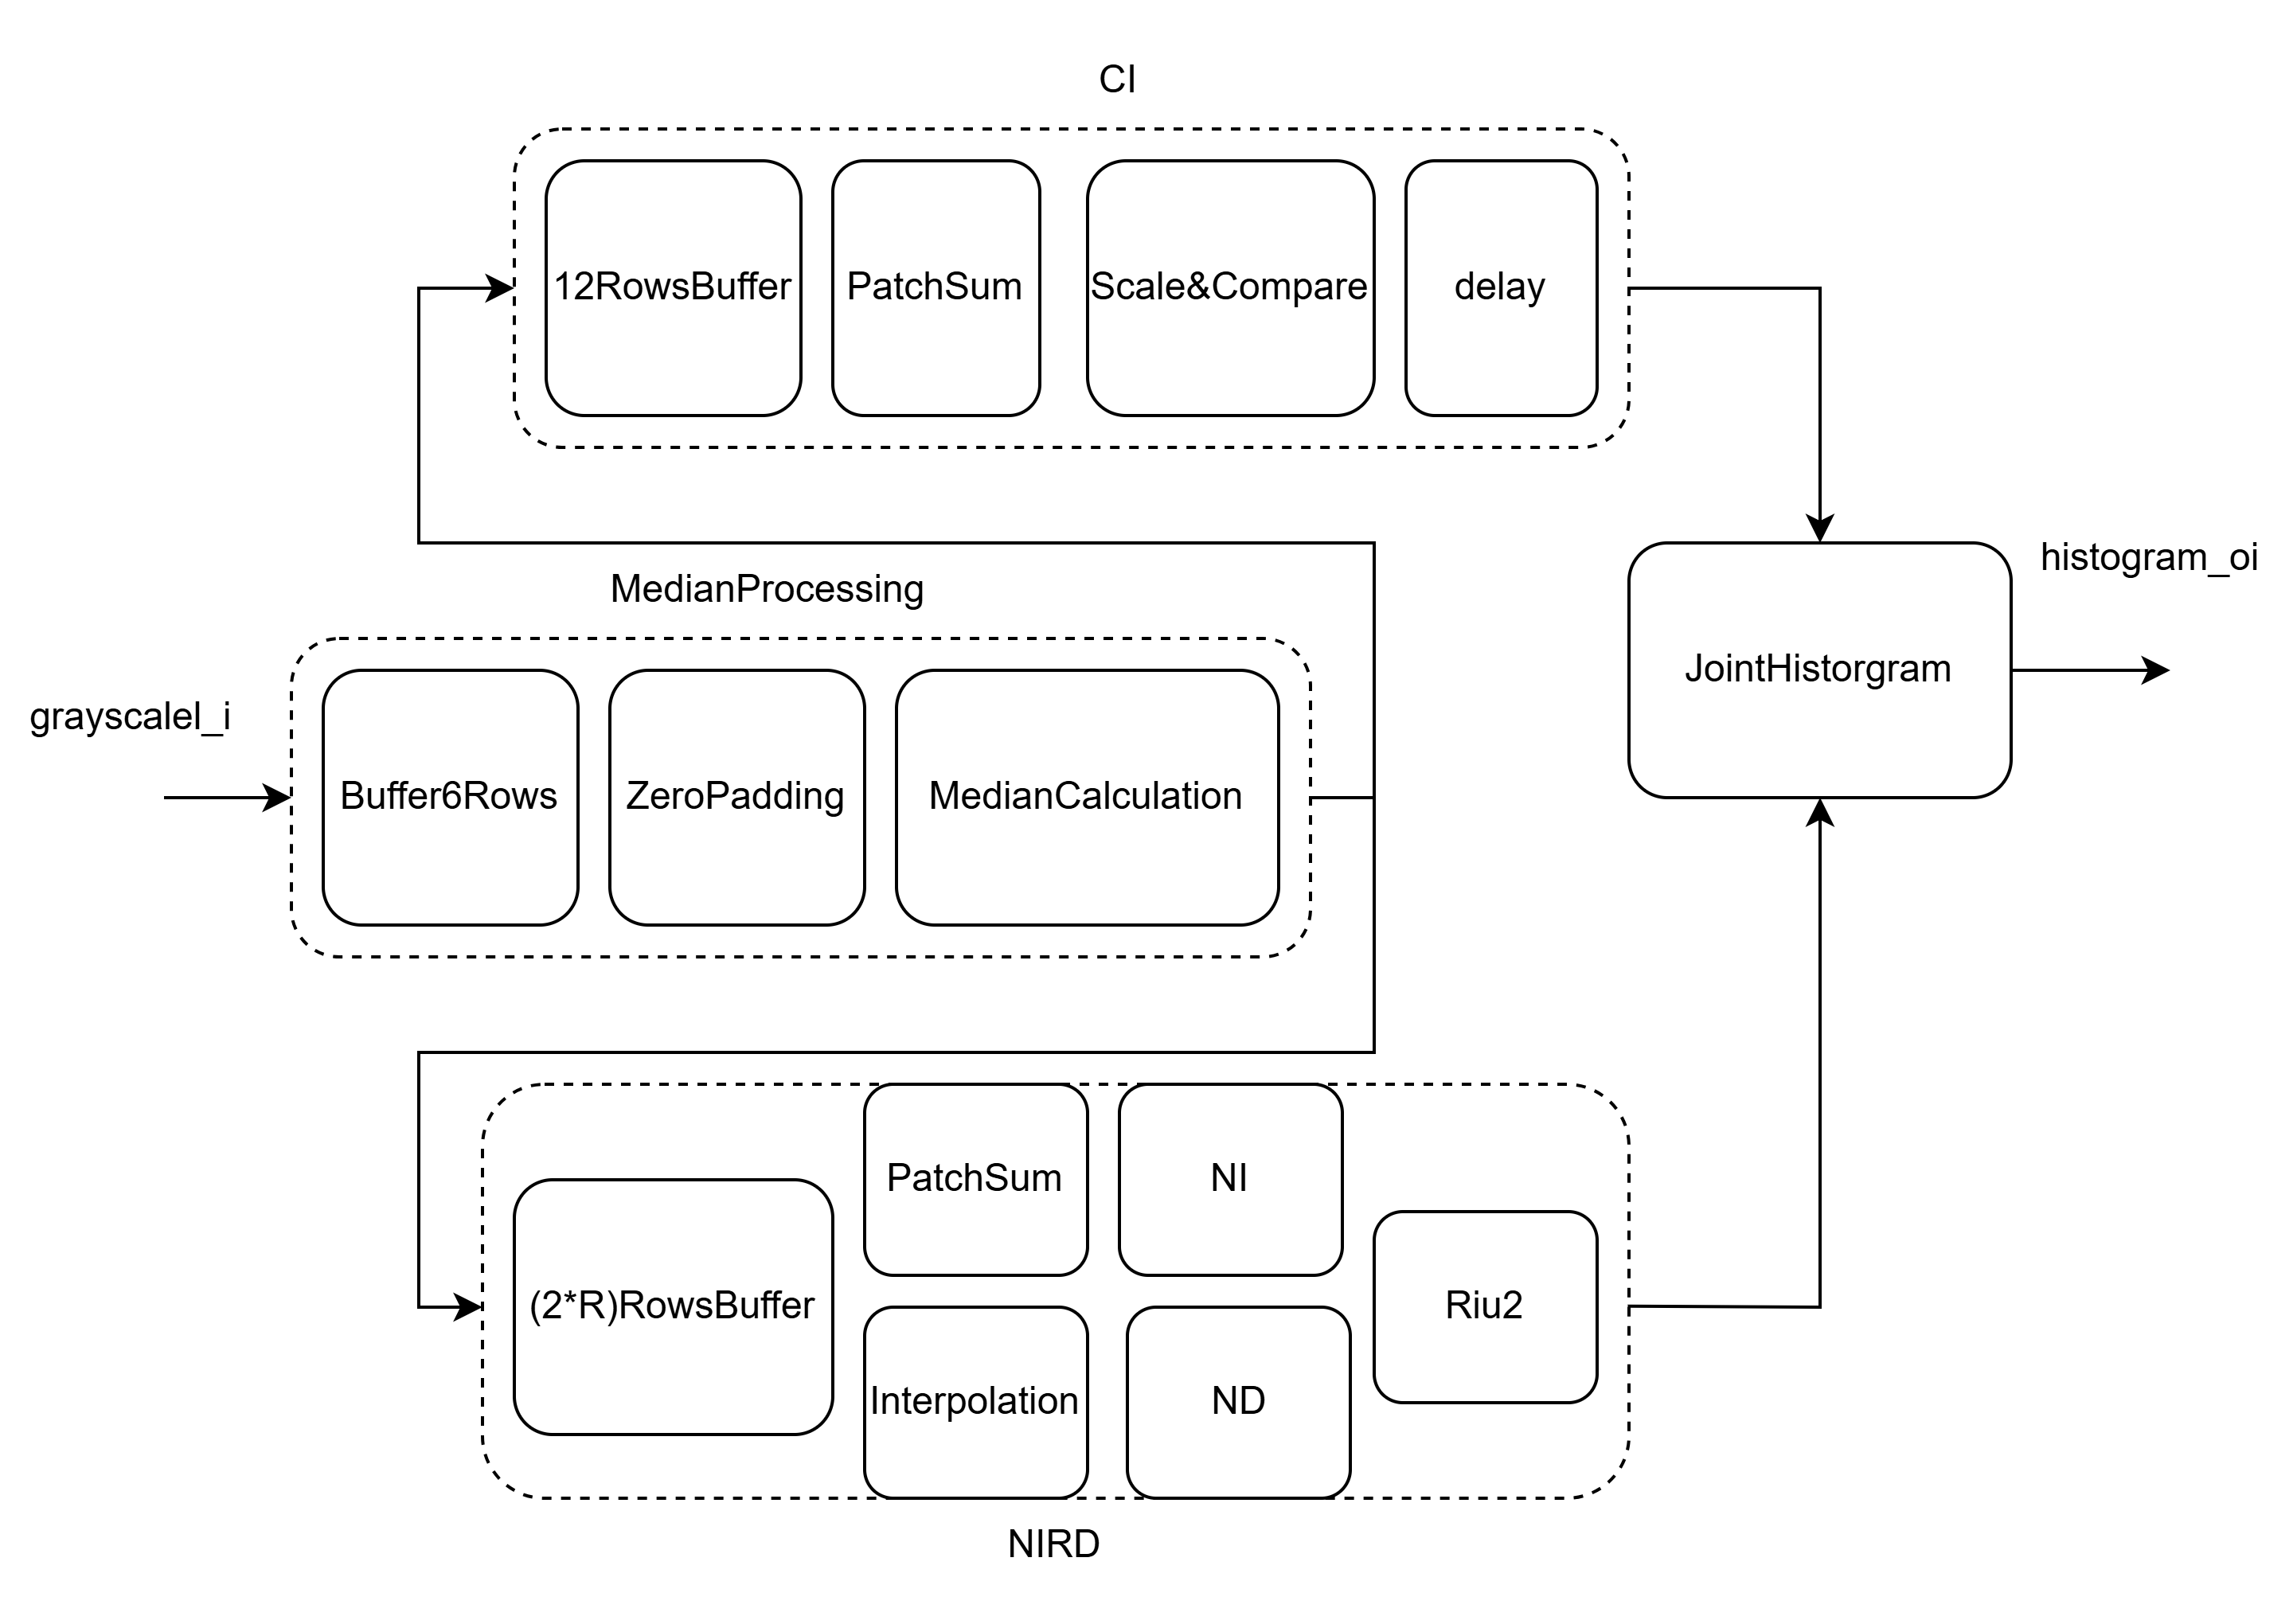
\includegraphics[width=1\linewidth]{figures/mrelbpArchitecture.png}
	\caption{Sơ đồ khối của mô-đun MRELBP}
	\label{fig:mrelbpArchitecture}
\end{figure}



\begin{figure} [!ht]
	\centering
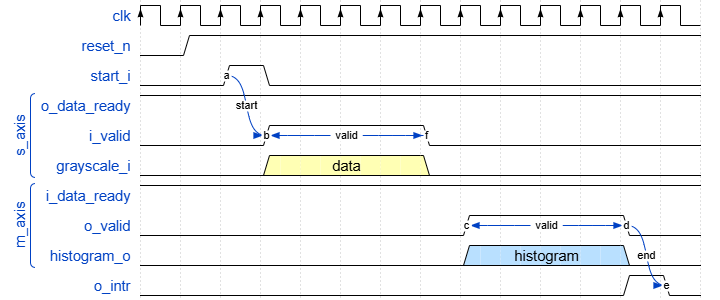
\includegraphics[width=1\linewidth]{figures/mrelbp.png}
	\caption{Dạng sóng của mô-đun MRELBP}
	\label{fig:mrelbpWaveform}
\end{figure}




\newpage
\subsection{Đặc tả mô-đun MedianProcessing}
Theo mô tả từ hình \ref{fig:mrelbpArchitecture} thì môn đun MedianProcessing gồm 3 thành phần chính hay 3 mô-đun bao gồm \textbf{Buffer6Rows, ZeroPadding, MedianCalculation}. \textit{\textbf{Lưu ý}: Do mô-đun MedianProcessing sẽ tính giá trị trung vị ứng với 3 cửa sổ theo bán kính r, nên tại phần này sẽ mô tả một cách tổng quát từng mô-đun mà không chi tiết cụ thể theo từng giá trị r}.
\begin{table}[!ht]
    \centering
    \renewcommand{\arraystretch}{1.3} % Tăng khoảng cách dòng
        \caption{Tham số của mô-đun MedianProcessing}
    \begin{tabular}{|p{3cm} p{4cm} p{8cm}|}
        \hline
        \rowcolor{gray!30}
        \textbf{Tham số } & \textbf{Giá trị mặc định}  & \textbf{Mô tả} \\
        \hline
        COLS & 128 & Kích thước độ rộng của ảnh
        \\ \hline
        ROWS & 128 & Kích thước chiều cao của ảnh
        \\
        \hline
    \end{tabular}

    \label{tab:paramListMedianProcessing}
\end{table}

\begin{table}[!ht]
    \centering
    \renewcommand{\arraystretch}{1.3} % Tăng khoảng cách dòng
        \caption{Danh sách các tín hiệu của mô-đun MedianProcessing}
    \begin{tabular}{|p{3cm} p{2cm} p{2cm} p{8cm}|}
        \hline
        \rowcolor{gray!30}
        \textbf{Tên tín hiệu} & \textbf{Độ rộng} & \textbf{Vào ra} & \textbf{Mô tả} \\
        \hline
        clk & 1 & Vào & Tín hiệu clock \\
        \hline
        rst\_n & 1 & Vào & Reset đồng bộ, kích hoạt mức thấp \\
        \hline 
        data\_i & 8 & Vào & Dữ liệu điểm ảnh đầu vào
        \\ \hline
        i\_valid & 1 & Vào & Tín hiệu thông báo giá trị đầu vào là hợp lệ
        \\ \hline
        data\_o & 8 & Ra & Dữ liệu điểm ảnh đầu ra gốc
        \\ \hline
        o\_valid & 1 & Ra & Tín hiệu thông báo dữ liệu đầu ra gốc là hợp lệ
        \\ \hline
        m\_3x3\_o & 8 & Ra & Giá trị trung vị của cửa sổ 3x3
        \\ \hline
        o\_3x3\_valid & 1 & Ra & Tín hiệu thông báo dữ liệu trung vị 3x3 hợp lệ
                \\ \hline
        m\_5x5\_o & 8 & Ra & Giá trị trung vị của cửa sổ 5x5
        \\ \hline
        o\_5x5\_valid & 1 & Ra & Tín hiệu thông báo dữ liệu trung vị 5x5 hợp lệ
                \\ \hline
        m\_7x7\_o & 8 & Ra & Giá trị trung vị của cửa sổ 7x7
        \\ \hline
        o\_7x7\_valid & 1 & Ra & Tín hiệu thông báo dữ liệu trung vị 7x7 hợp lệ
        \\ \hline
       
    \end{tabular}

    \label{tab:signalListMedianProcessing}
\end{table}

\begin{figure}[!ht]
    \centering
    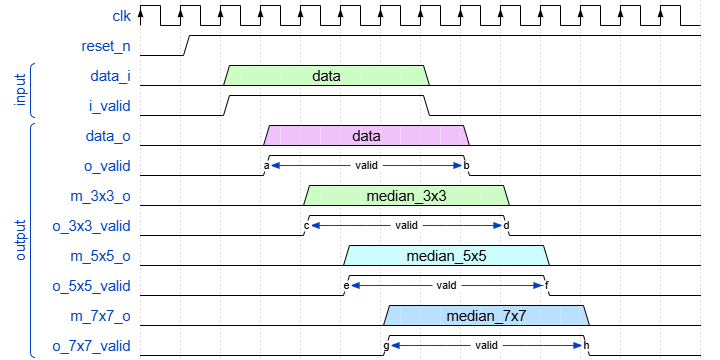
\includegraphics[width=1\linewidth, height =7cm]{figures/medianProcessing.png}
    \caption{Dạng sóng của mô-đun MedianProcessing}
    \label{fig:medianProcessing}
\end{figure}
\subsubsection{Đặc tả mô-đun Buffer6Rows}
mô-đun Buffer6Rows là tập hợp của \textbf{6} mô-đun LineBuffer tạo thành, cụ thể được mô tả trong hình \ref{fig:buffer6RowsAr}. Do đó, để mô tả đặc tả cho mô-đun Buffer6Rows, ta sẽ đi từ mô-đun LineBuffer. mô-đun LineBuffer là mô-đun cơ sở để xây dựng lên các mô-đun lớn hơn như Buffer6Rows. Chức năng của mô-đun này là đệm dữ liệu theo từng hàng để thuận tiện cho việc định dạng dữ liệu cho các mô-đun đứng sau.

\begin{figure}[!ht]
    \centering
    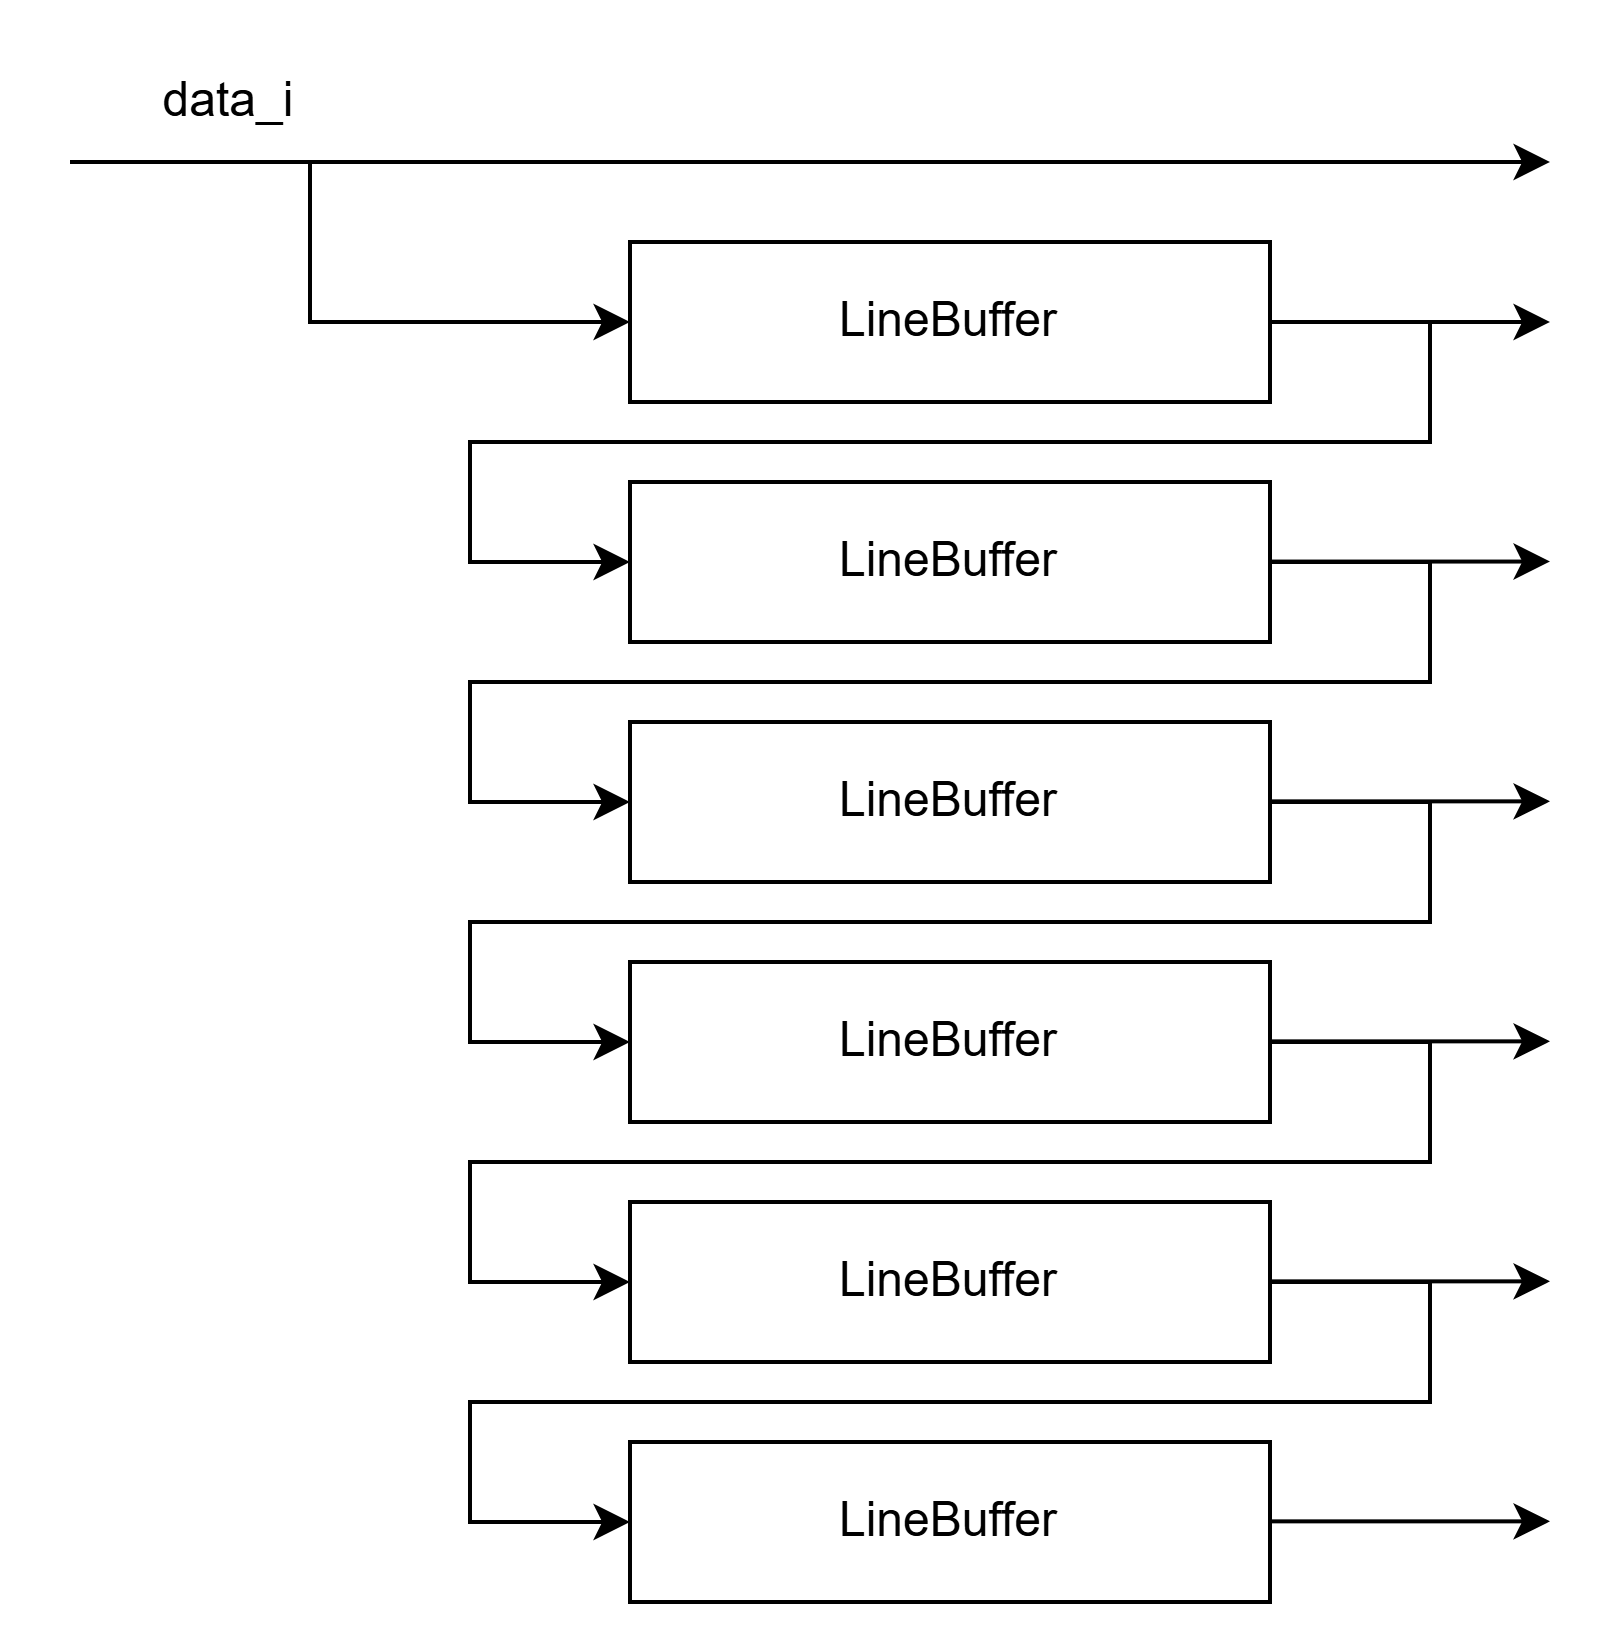
\includegraphics[width=1\linewidth]{figures/buffer6RowsAr.png}
    \caption{Sơ đồ khối của mô-đun Buffer6Rows}
    \label{fig:buffer6RowsAr}
\end{figure}


\begin{table}[!ht]
    \centering
    \renewcommand{\arraystretch}{1.3} % Tăng khoảng cách dòng
        \caption{Danh sách các tham số của mô-đun LineBuffer }
    \begin{tabular}{|p{3cm} p{4cm} p{8cm}|}
        \hline
        \rowcolor{gray!30}
        \textbf{Tham số } & \textbf{Giá trị mặc định}  & \textbf{Mô tả} \\
        \hline
        DEPTH & 128 & Kích thước độ rộng của ảnh
        \\ \hline
    \end{tabular}

    \label{tab:paramListLineBuffer}
\end{table}


\begin{table}[h]
    \centering
    \renewcommand{\arraystretch}{1.3} % Tăng khoảng cách dòng
        \caption{Danh sách các tín hiệu của giao diện mô-đun LineBuffer}
    \begin{tabular}{|p{3cm} p{2cm} p{2cm} p{8cm}|}
        \hline
        \rowcolor{gray!30}
        \textbf{Tên tín hiệu} & \textbf{Độ rộng} & \textbf{Vào ra} & \textbf{Mô tả} \\
        \hline
        clk & 1 & Vào & Tín hiệu clock \\
        \hline
        rst\_n & 1 & Vào & Reset đồng bộ, kích hoạt mức thấp \\
        \hline
        i\_valid & 1 & Vào & Tín hiệu thông báo dữ liệu đầu vào là hợp lệ
        \\ \hline
        data\_i & 8 & Vào & Dữ liệu đầu vào
        \\ \hline
        data\_o & 8 & Ra & Dữ liệu đầu ra
        \\ \hline
        o\_start & 1& Ra & Tín hiệu thông báo bắt đầu có dữ liệu đầu ra
        \\ \hline
        o\_valid & 1& Ra & Tín hiệu thông báo dữ liệu đầu là hợp lệ
        \\ \hline
        o\_finish & 1 & Ra & Tín hiệu thông báo kết thúc đệm dữ liệu        
        \\ \hline
    \end{tabular}

    \label{tab:signalListLineBuffer}
\end{table}
\begin{figure}[!ht]
    \centering
    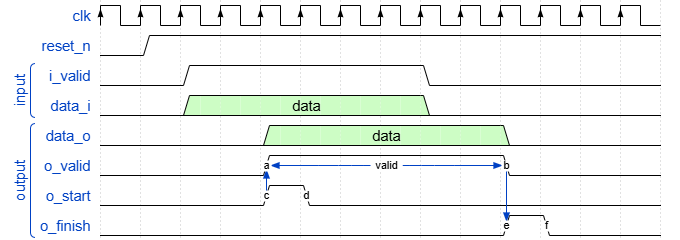
\includegraphics[width=1\linewidth]{figures/lineBuffer.png}
    \caption{Dạng sóng của mô-đun LineBuffer}
    \label{fig:lineBuffer}
\end{figure}
\begin{figure}[!ht]
    \centering
    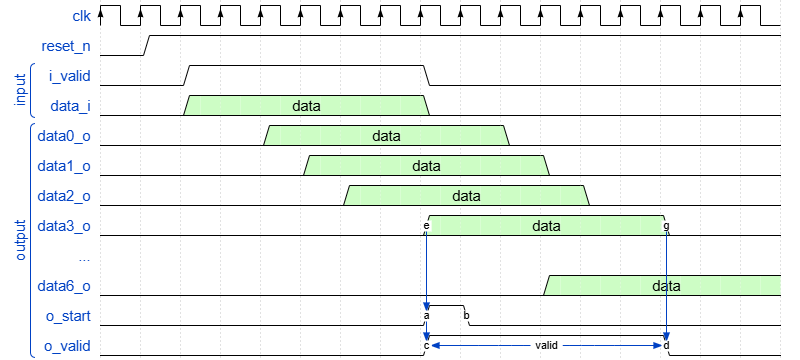
\includegraphics[width=1\linewidth]{figures/Buffer6Rows.png}
    \caption{Dạng sóng của mô-đun Buffer6Rows}
    \label{fig:Buffer6Rows}
\end{figure}

\subsubsection{Đặc tả mô-đun ZeroPadding}
Đệm 0 là một kỹ thuật được sử dụng để thêm hàng và cột vào rìa bức ảnh, mục đích để khi xử lý với một số kỹ thuật như nhân chập, kích thước đầu ra sẽ không bị thay đổi so với đầu vào \textit{(danh sách tín hiệu sẽ có mô tả chung về số lượng đầu vào\&ra vì các tín hiệu cửa mô-đun sẽ thuộc vào kích thước cửa sổ, xem thêm ở phần RTL của ZeroPadding).}




\begin{table}[!ht]
    \centering
    \renewcommand{\arraystretch}{1.3} % Tăng khoảng cách dòng
        \caption{Danh sách các tham số của mô-đun ZeroPadding }
    \begin{tabular}{|p{3cm} p{4cm} p{8cm}|}
        \hline
        \rowcolor{gray!30}
        \textbf{Tham số } & \textbf{Giá trị mặc định}  & \textbf{Mô tả} \\
        \hline
        COLS & 128 & Kích thước độ rộng của ảnh
        \\ \hline
        ROWS & 128 & Kích thước độ cao của ảnh
        \\ \hline
    \end{tabular}

    \label{tab:paramListZeroPadding}
\end{table}


\begin{table}[h]
    \centering
    \renewcommand{\arraystretch}{1.3} % Tăng khoảng cách dòng
        \caption{Danh sách các tín hiệu của giao diện mô-đun ZeroPadding}
    \begin{tabular}{|p{3cm} p{2cm} p{2cm} p{8cm}|}
        \hline
        \rowcolor{gray!30}
        \textbf{Tên tín hiệu} & \textbf{Độ rộng} & \textbf{Vào ra} & \textbf{Mô tả} \\
        \hline
        clk & 1 & Vào & Tín hiệu clock \\
        \hline
        rst\_n & 1 & Vào & Reset đồng bộ, kích hoạt mức thấp \\
        \hline
        i\_valid & 1 & Vào & Tín hiệu thông báo dữ liệu đầu vào là hợp lệ
        \\ \hline
        d0\_i & 8 & Vào & Dữ liệu đầu vào
        \\ \hline
        d1\_i & 8 & Vào & Dữ liệu đầu vào
        \\
        \hline
        \multicolumn{4}{|c|}{Tùy thuộc vào kích thước cửa sổ, 3x3 thì sẽ có 3 đầu vào, 5x5 có 5 đầu vào, 7x7 có 7 đầu vào}
        \\ \hline
        d0\_o & 8 & Ra & Dữ liệu đầu ra
        \\ \hline
        d1\_o & 8 & Ra & Dữ liệu đầu ra
        \\ \hline
                \multicolumn{4}{|c|}{Tùy thuộc vào kích thước cửa sổ, 3x3 thì sẽ có 9 đầu ra, 5x5 có 25 đầu ra, 7x7 có 49 đầu ra}
        \\ \hline
        o\_valid & 1& Ra & Tín hiệu thông báo dữ liệu đầu là hợp lệ
        \\ \hline
    \end{tabular}

    \label{tab:signalListZeroPadding}
\end{table}

\begin{figure}[!ht]
    \centering
    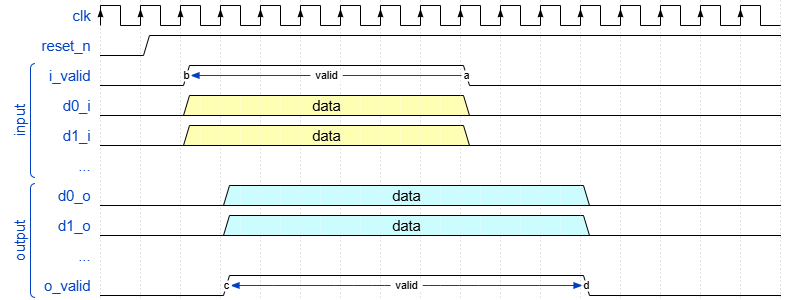
\includegraphics[width=\linewidth]{figures/zeroPadding.png}
    \caption{Dạng sóng của mô-đun ZeroPadding}
    \label{fig:zeroPadding}
\end{figure}


\subsubsection{Đặc tả mô-đun MedianCalculation}
Vì kiến trúc của mô-đun MedianCalculation sẽ phụ thuộc vào từng loại cửa sổ, tức là cửa sổ 3x3 sẽ có cách tính khác cửa sổ 5x5, nên để thuận lợi cho việc mô tả, sinh viên sẽ mô tả theo 1 giao diện chung mà số lượng các cổng sẽ khác đối với từng loại cửa sổ. Cụ thể hơn sẽ được mô tả tại thiết kế RTL cho mô-đun MedianCalculation
\begin{table}[!ht]
    \centering
    \renewcommand{\arraystretch}{1.3} % Tăng khoảng cách dòng
        \caption{Danh sách các tham số của mô-đun MedianCalculation}
    \begin{tabular}{|p{3cm} p{4cm} p{8cm}|}
        \hline
        \rowcolor{gray!30}
        \textbf{Tham số } & \textbf{Giá trị mặc định}  & \textbf{Mô tả} \\
        \hline
        COLS & 128 & Kích thước độ rộng của ảnh
        \\ \hline
        ROWS & 128 & Kích thước độ cao của ảnh
        \\ \hline
    \end{tabular}

    \label{tab:paramListMedianCalculation}
\end{table}


\begin{table}[h]
    \centering
    \renewcommand{\arraystretch}{1.3} % Tăng khoảng cách dòng
        \caption{Danh sách các tín hiệu của giao diện mô-đun MedianCalculation}
    \begin{tabular}{|p{3cm} p{2cm} p{2cm} p{8cm}|}
        \hline
        \rowcolor{gray!30}
        \textbf{Tên tín hiệu} & \textbf{Độ rộng} & \textbf{Vào ra} & \textbf{Mô tả} \\
        \hline
        clk & 1 & Vào & Tín hiệu clock \\
        \hline
        rst\_n & 1 & Vào & Reset đồng bộ, kích hoạt mức thấp \\
        \hline
        i\_valid & 1 & Vào & Tín hiệu thông báo dữ liệu đầu vào là hợp lệ
        \\ \hline
        S0\_i & 8 & Vào & Dữ liệu đầu vào
        \\ \hline
        S1\_i & 8 & Vào & Dữ liệu đầu vào
        \\
        \hline
        \multicolumn{4}{|c|}{Tùy thuộc vào kích thước cửa sổ, 3x3 thì sẽ có 9 đầu vào, 5x5 có 25 đầu vào, 7x7 có 49 đầu vào}
        \\ \hline
        median\_o & 8 & Ra & Dữ liệu đầu ra
        \\ \hline
        o\_valid & 1& Ra & Tín hiệu thông báo dữ liệu đầu là hợp lệ
        \\ \hline
    \end{tabular}

    \label{tab:signalListMedianCalculation}
\end{table}

\begin{figure}[!ht]
    \centering
    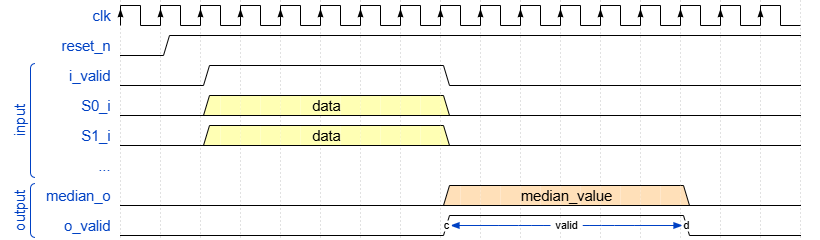
\includegraphics[width=\linewidth]{figures/medianCalculation.png}
    \caption{Dạng sóng của mô-đun MedianCalculation}
    \label{fig:medianCalculation}
\end{figure}
\subsection{Đặc tả mô-đun CI}
Bảng \ref{tab:paramListCI}, \ref{tab:signalListCI} mô tả các tham số và tín hiệu đầu vào, đầu ra của mô-đun CI.

\begin{table}[!ht]
    \centering
    \renewcommand{\arraystretch}{1.3} % Tăng khoảng cách dòng
        \caption{Tham số của mô-đun CI}
    \begin{tabular}{|p{3cm} p{4cm} p{8cm}|}
        \hline
        \rowcolor{gray!30}
        \textbf{Tham số } & \textbf{Giá trị mặc định}  & \textbf{Mô tả} \\
        \hline
        COLS & 128 & Kích thước độ rộng của ảnh
        \\ \hline
        ROWS & 128 & Kích thước chiều cao của ảnh
        \\
        \hline
    \end{tabular}

    \label{tab:paramListCI}
\end{table}

\begin{table}[!ht]
    \centering
    \renewcommand{\arraystretch}{1.3} % Tăng khoảng cách dòng
        \caption{Danh sách các tín hiệu của mô-đun CI}
    \begin{tabular}{|p{3cm} p{2cm} p{2cm} p{8cm}|}
        \hline
        \rowcolor{gray!30}
        \textbf{Tên tín hiệu} & \textbf{Độ rộng} & \textbf{Vào ra} & \textbf{Mô tả} \\
        \hline
        clk & 1 & Vào & Tín hiệu clock \\
        \hline
        rst\_n & 1 & Vào & Reset đồng bộ, kích hoạt mức thấp \\
        \hline 
        m\_3x3\_i & 8 & Vào & Dữ liệu trung vị của cửa sổ 3x3
        \\ \hline
        ci\_r2\_o & 1 & Ra & Mô tả ci đầu ra ứng với r = 2
        \\ \hline
        r2\_valid & 1 & Ra & Tín hiệu thông báo ci ứng với r = 2 là hợp lệ
        \\ \hline
        r2\_finish & 1 & Ra & Tín hiệu thông báo đã kết thúc quá trình tính ci ứng với r = 2
        \\ \hline
                ci\_r4\_o & 1 & Ra & Mô tả ci đầu ra ứng với r = 4
        \\ \hline
        r4\_valid & 1 & Ra & Tín hiệu thông báo ci ứng với r = 4 là hợp lệ
        \\ \hline
        r4\_finish & 1 & Ra & Tín hiệu thông báo đã kết thúc quá trình tính ci ứng với r = 4
        \\ \hline
                ci\_r6\_o & 1 & Ra & Mô tả ci đầu ra ứng với r = 6
        \\ \hline
        r6\_valid & 1 & Ra & Tín hiệu thông báo ci ứng với r = 6 là hợp lệ
        \\ \hline
        r6\_finish & 1 & Ra & Tín hiệu thông báo đã kết thúc quá trình tính ci ứng với r = 6
        \\ \hline
       
    \end{tabular}

    \label{tab:signalListCI}
\end{table}

\begin{figure}[!ht]
    \centering
    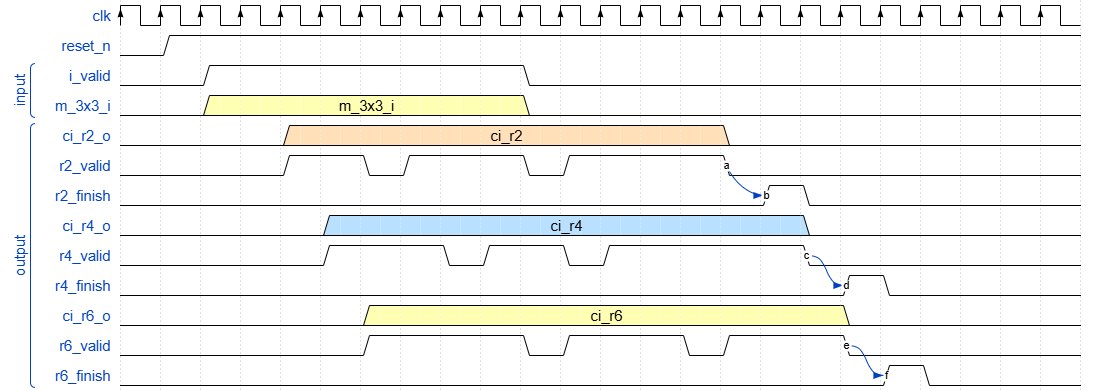
\includegraphics[width=\linewidth]{figures/ci.png}
    \caption{Dạng sóng của mô-đun CI}
    \label{fig:ci}
\end{figure}

Hình \ref{fig:ciArch} mô tả kiến trúc tổng quát của mô-đun CI. Sau khi giá trị trung vị tính từ cửa sổ 3x3 được tính xong sẽ đưa vào mô-đun này. Trong đây sẽ cần một bộ 12RowsBuffer để đệm dữ liệu nhằm tạo cửa sổ cho khối sau sử dụng với kích thước là (2*r+1, 2*r+1), vì r = 6 nên cửa sổ lớn nhất là 13x13, do đó nên cần đệm 12 hàng. Dữ liệu sau khi đệm sẽ đưa vào một khối gọi là "PatchSum", khối này có nhiệm vụ ghép dữ liệu thành một cửa sổ, sử dụng kĩ thuật cửa sổ trượt để tính tổng của cửa sổ và đầu ra sẽ bao gồm tổng và giá trị ở giữa của cửa sổ. Sau đó khối compare là mạch logic tổ hợp có thể so sánh và đưa ra giá trị CI ứng với cửa sổ đang được tính. Hình \ref{fig:mrelbpArchitecture} có mô tả thêm khối \textbf{"delay"}, thì khối này thực tế để làm trễ dữ liệu CI đầu ra để đồng bộ với NIRD, thực tế nó là các thanh ghi dịch, do đó sẽ không trình bày phần delay này. mô-đun 12RowsBuffer có nguyên tắc hoạt động tương tự với mô-đun Buffer6Rows. Phần gộp vào giữa PatchSum và khối logic tổ hợp gọi là \textit{MRELBP\_CI}. 

\begin{figure}[!ht]
    \centering
    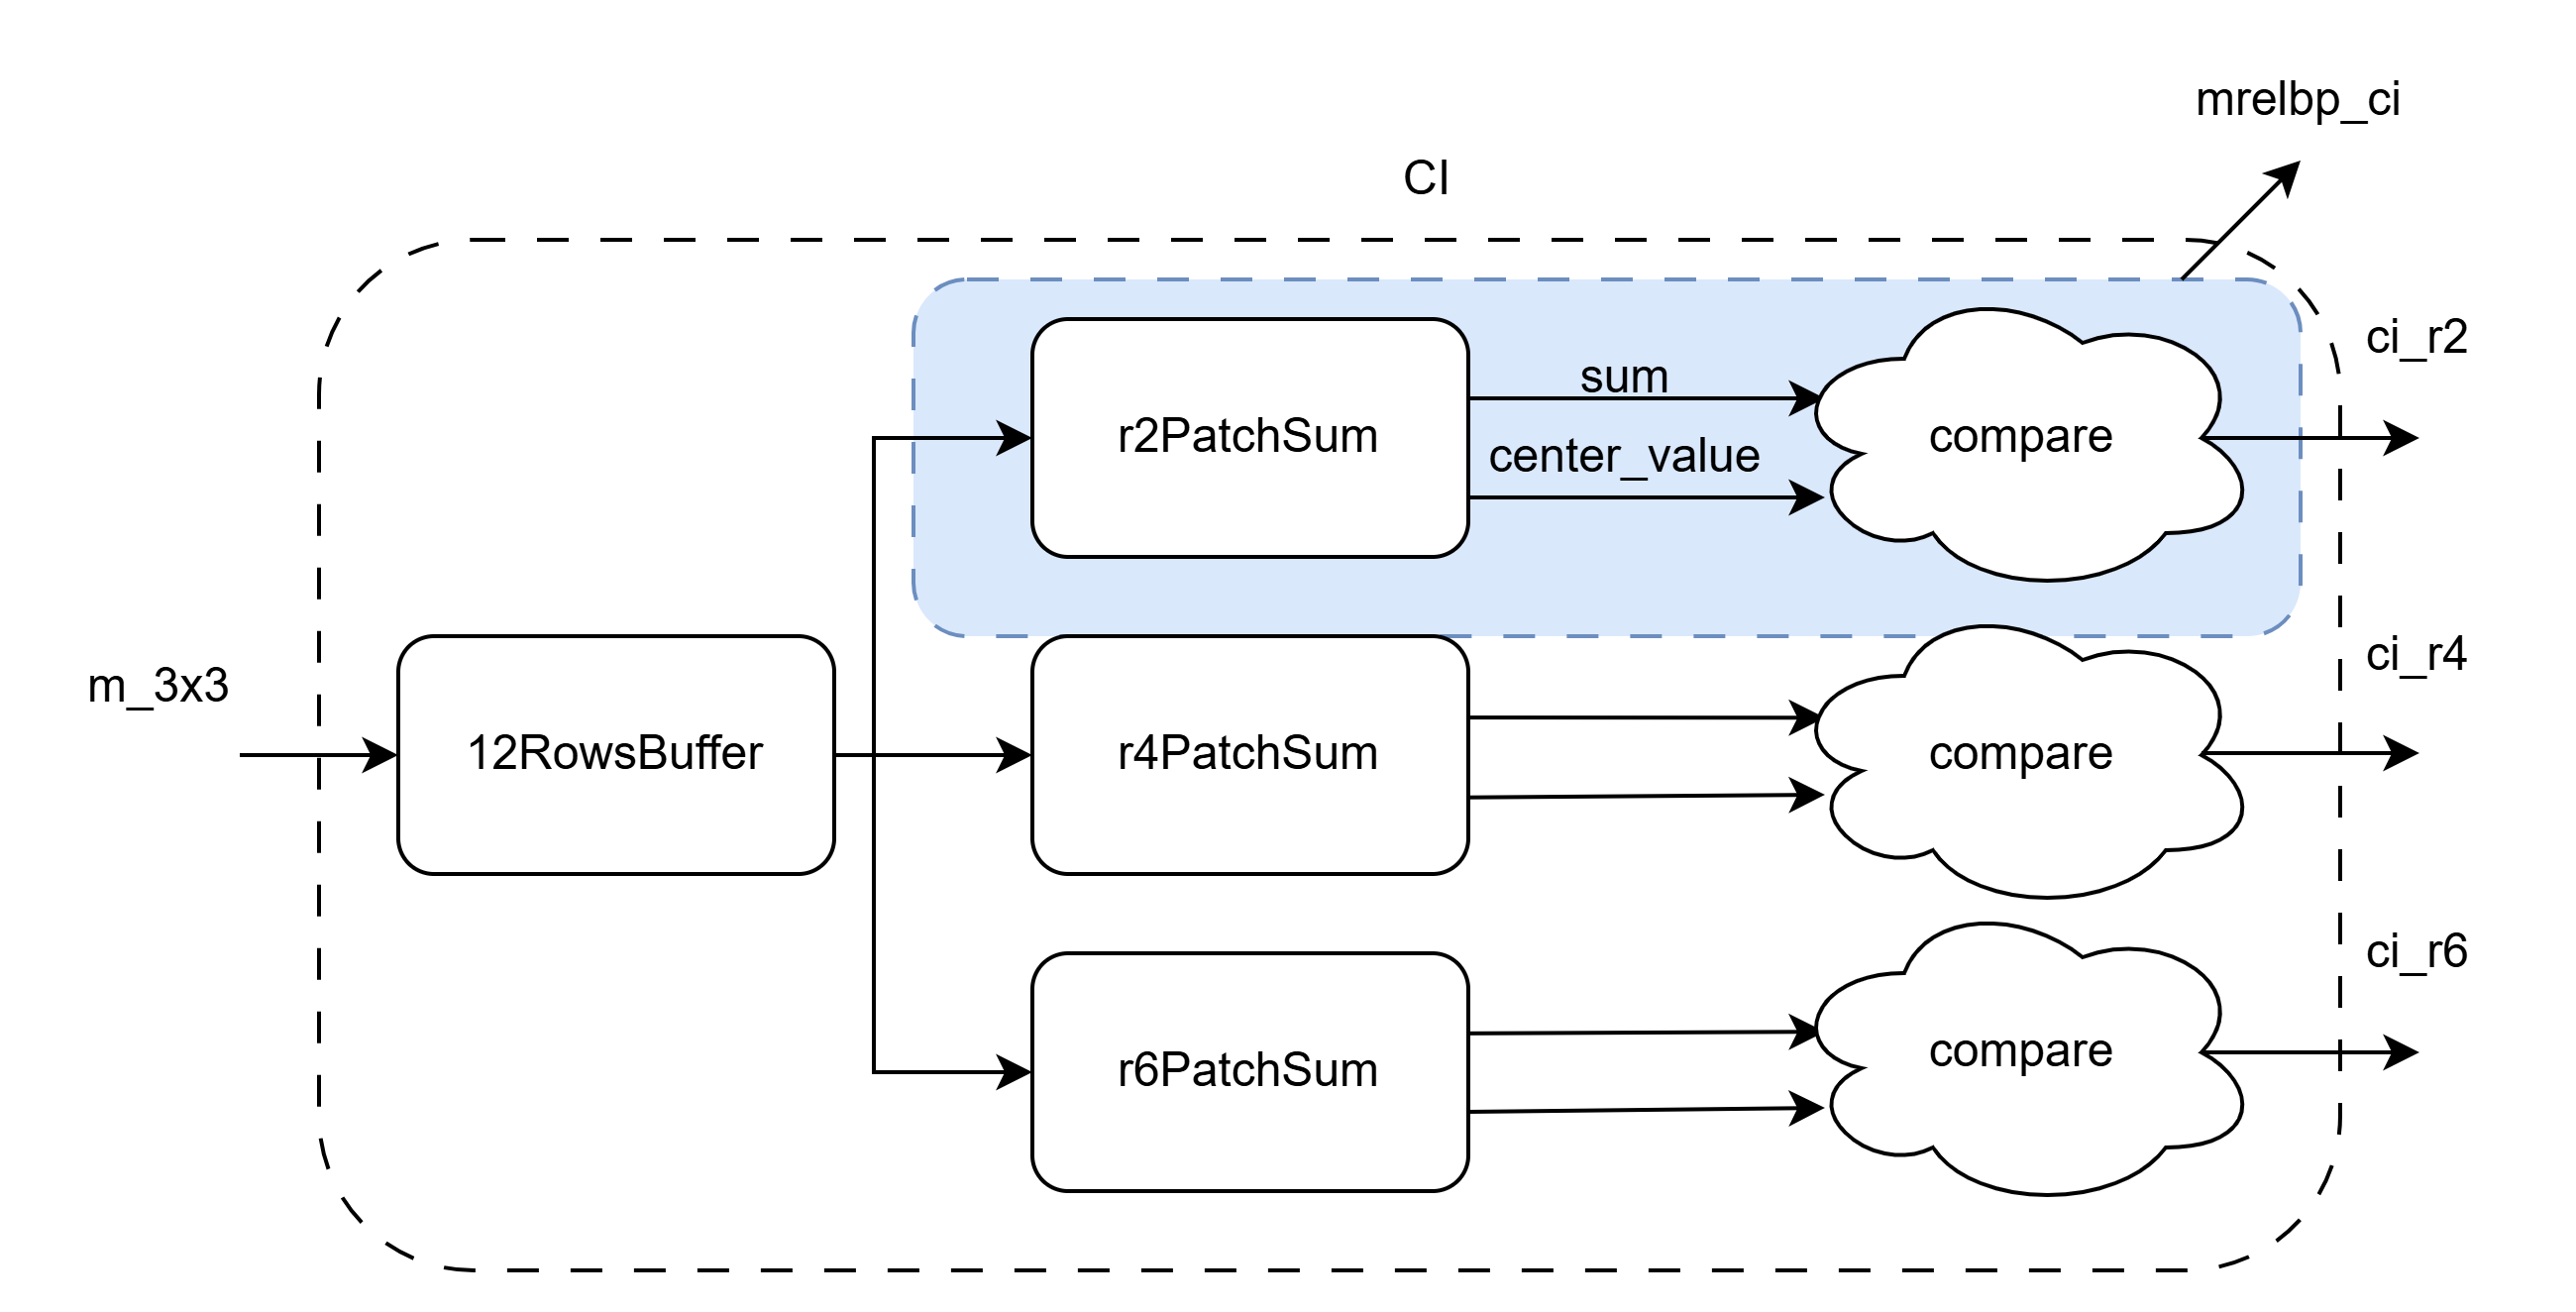
\includegraphics[width=\linewidth]{figures/ciArch.png}
    \caption{Sơ đồ khối của mô-đun CI}
    \label{fig:ciArch}
\end{figure}

\subsubsection{Đặc tả mô-đun MRELBP\_CI}
Bảng \ref{tab:paramListCICAL}, \ref{tab:signalListCICAL} mô tả về giao diện kết nối của mô-đun MRELBP\_CI. Với mô-đun này, sẽ được thiết kế theo nhiều giá trị r, ứng với đó thì sẽ có số lượng đầu vào khác nhau. Đầu ra gồm tín hiệu ci\_o, tín hiệu này chỉ có 1-bit ứng với 2 giá trị có thể có là 0 hoặc 1. Theo hình \ref{fig:ciArch}, bên trong mô-đun này sẽ có mô-đun \textit{PatchSum} để tính toán tổng của các điểm ảnh trong cửa sổ và sau đó là một khối logic tổ hợp để so sánh giá trị của \textbf{sum} và \textbf{center\_value} tương ứng với tổng của cửa sổ và điểm ảnh nằm giữa của cửa sổ. Chi tiết hơn sẽ được mô tả tại thiết kế RTL của mô-đun MRELBP\_CI. 


\begin{table}[!ht]
    \centering
    \renewcommand{\arraystretch}{1.3} % Tăng khoảng cách dòng
        \caption{Tham số của mô-đun MRELBP\_CI}
    \begin{tabular}{|p{3cm} p{4cm} p{8cm}|}
        \hline
        \rowcolor{gray!30}
        \textbf{Tham số } & \textbf{Giá trị mặc định}  & \textbf{Mô tả} \\
        \hline
        COLS & 128 & Kích thước độ rộng của ảnh
        \\ \hline
        ROWS & 128 & Kích thước chiều cao của ảnh
        \\
        \hline
    \end{tabular}

    \label{tab:paramListCICAL}
\end{table}
\begin{table}[!ht]
    \centering
    \renewcommand{\arraystretch}{1.3} % Tăng khoảng cách dòng
    \caption{Danh sách các tín hiệu của mô-đun MRELBP\_CI}
    \begin{tabular}{|p{3cm} p{2cm} p{2cm} p{8cm}|}
        \hline
        \rowcolor{gray!30}
        \textbf{Tên tín hiệu} & \textbf{Độ rộng} & \textbf{Vào ra} & \textbf{Mô tả} \\
        \hline
        clk & 1 & Vào & Tín hiệu clock \\
        \hline
        rst\_n & 1 & Vào & Reset đồng bộ, kích hoạt mức thấp \\
        \hline 
        i\_valid & 1 & Vào & Tín hiệu thông báo dữ liệu đầu vào là hợp lệ
        \\ \hline
        S1\_i & 8 & Vào & Dữ liệu đầu vào 1
        \\ \hline
        S2\_i & 8 & Vào & Dữ liệu đầu vào 2
        \\ \hline
                S3\_i & 8 & Vào & Dữ liệu đầu vào 3
        \\ \hline
                S4\_i & 8 & Vào & Dữ liệu đầu vào 4
        \\ \hline
                        S5\_i & 8 & Vào & Dữ liệu đầu vào 5
        \\ \hline
        \multicolumn{4}{|c|}{Tùy thuộc vào giá trị bán kính, r = 2 thì sẽ có 5 đầu vào, r = 4 có 9 đầu vào vào, r = 6 có 13 đầu vào}
        \\ \hline
        ci\_o & 1 & Ra & Mô tả CI đầu ra
        \\ \hline
        o\_valid & 1 & Ra & Tín hiêu thông báo dữ liệu đầu ra là hợp lệ
        \\ \hline
        o\_finish & 1 & Ra & Tín hiệu thông báo kết thúc quá trình tính CI
        \\ \hline
       
    \end{tabular}

    \label{tab:signalListCICAL}
\end{table}
\begin{figure}[!ht]
    \centering
    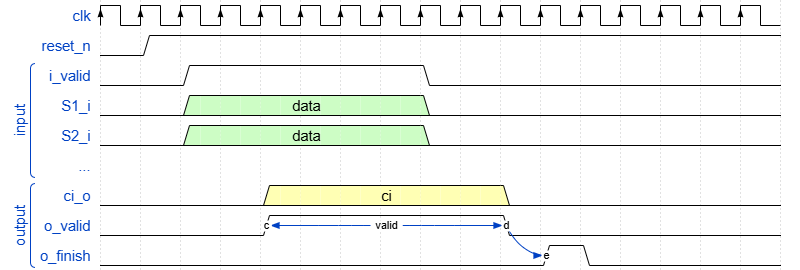
\includegraphics[width=\linewidth]{figures/mrelbpCI.png}
    \caption{Dạng sóng của mô-đun MRELBP\_CI}
    \label{fig:mrelbpCIl}
\end{figure}
\newpage
\subsection{Đặc tả mô-đun NIRD}

Hình \ref{fig:nirdArch} mô tả sơ đồ khối của mô-đun NIRD. Tại mô-đun này ta cần tính hai mô tả là NI và RD theo công thức \ref{eq:relbp_ni} và \ref{eq:relbp_rd}. Vì khi tính RD cần tham chiếu đến hai cửa sổ kích thước khác nhau và dữ liệu của điểm ảnh cũng là đầu ra của bộ lọc trung vị cửa sổ khác nhau, do đó đầu vào sẽ có 2 dữ liệu ứng bán kính r và r1 với r1 = r - 1. Dữ liệu cũng sẽ cần được đệm qua hai bộ đệm có số lượng mô-đun LineBuffer bằng 2*r với r có thể là 2, 4, 6. Sau đó sẽ đi đến mô-đun WindowBuffer với mục đích để hình thành các cửa sổ dữ liệu để thuận lợi cho việc tính toán của các mô-đun sau. Khi tính mô tả NI sẽ là so sánh 8 giá trị trong đường tròn bán kính r so với trung bình tổng bán kính của cửa sổ, do đó sẽ có đầu vào là tổng điểm ảnh của cửa sổ và 8 điểm ảnh trong đường tròn bán kính r. 8 điểm ảnh này sẽ có 4 điểm cần phải suy ra bằng phương pháp nội suy. Với mô tả RD sẽ là so sánh của 8 điểm ảnh đường tròn bán kính r và 8 điểm ảnh trong đường tròn bán kính r1. Dữ liệu sau khi đạt được sẽ cần thực hiện một thao tác gọi là RIU2-mapping hay ánh xạ RIU2. Thực tế, mô-đun này sẽ làm nhiệm vụ chuyển 8-bit có được sau mô-đun NI hoặc RD thành một dạng biểu diễn khác ít bit hơn và mang nhiều ý nghĩa về mặt đặc trưng. Lý thuyết RIU2 đã được trình bày ở tiểu mục \ref{sec:lbp}.

\begin{table}[!ht]
    \centering
    \renewcommand{\arraystretch}{1.3} % Tăng khoảng cách dòng
        \caption{Tham số của mô-đun NIRD}
    \begin{tabular}{|p{3cm} p{4cm} p{8cm}|}
        \hline
        \rowcolor{gray!30}
        \textbf{Tham số } & \textbf{Giá trị mặc định}  & \textbf{Mô tả} \\
        \hline
        COLS & 128 & Kích thước độ rộng của ảnh
        \\ \hline
        ROWS & 128 & Kích thước chiều cao của ảnh
        \\
        \hline
    \end{tabular}

    \label{tab:paramListNIRD}
\end{table}
\begin{table}[!ht]
    \centering
    \renewcommand{\arraystretch}{1.3} % Tăng khoảng cách dòng
        \caption{Danh sách các tín hiệu của mô-đun NIRD}
    \begin{tabular}{|p{3cm} p{2cm} p{2cm} p{8cm}|}
        \hline
        \rowcolor{gray!30}
        \textbf{Tên tín hiệu} & \textbf{Độ rộng} & \textbf{Vào ra} & \textbf{Mô tả} \\
        \hline
        clk & 1 & Vào & Tín hiệu clock \\
        \hline
        rst\_n & 1 & Vào & Reset đồng bộ, kích hoạt mức thấp \\
        \hline 
        data\_r\_i & 8  & Vào &  Dữ liệu vào ứng với bán kính r
        \\ \hline
        i\_r\_valid & 1 & Vào & Tín hiệu thông báo dữ liệu đầu vào bán kính r hợp lệ
        \\ \hline
        data\_r1\_i & 8 & Vào & Dữ liệu vào ứng với bán kính r1
        \\ \hline
        i\_r1\_valid & 1 & Vào & Tín hiệu thông báo dữ liệu vào bán kính r1 hợp lệ
        \\ \hline
        ni\_o & 4 & Ra & Giá trị mô tả NI đầu ra
        \\ \hline
        rd\_o & 4 & Ra & Giá trị mô tả RD đầu ra
        \\ \hline
        o\_valid & 1 & Ra & Tín hiệu thông báo đầu ra là hợp lệ
        \\ \hline
        o\_finish & 1 & Ra & Tín hiệu thông báo kết thúc đầu ra
        \\ \hline
       
    \end{tabular}

    \label{tab:signalListNIRD}
\end{table}

\begin{figure}[!ht]
    \centering
    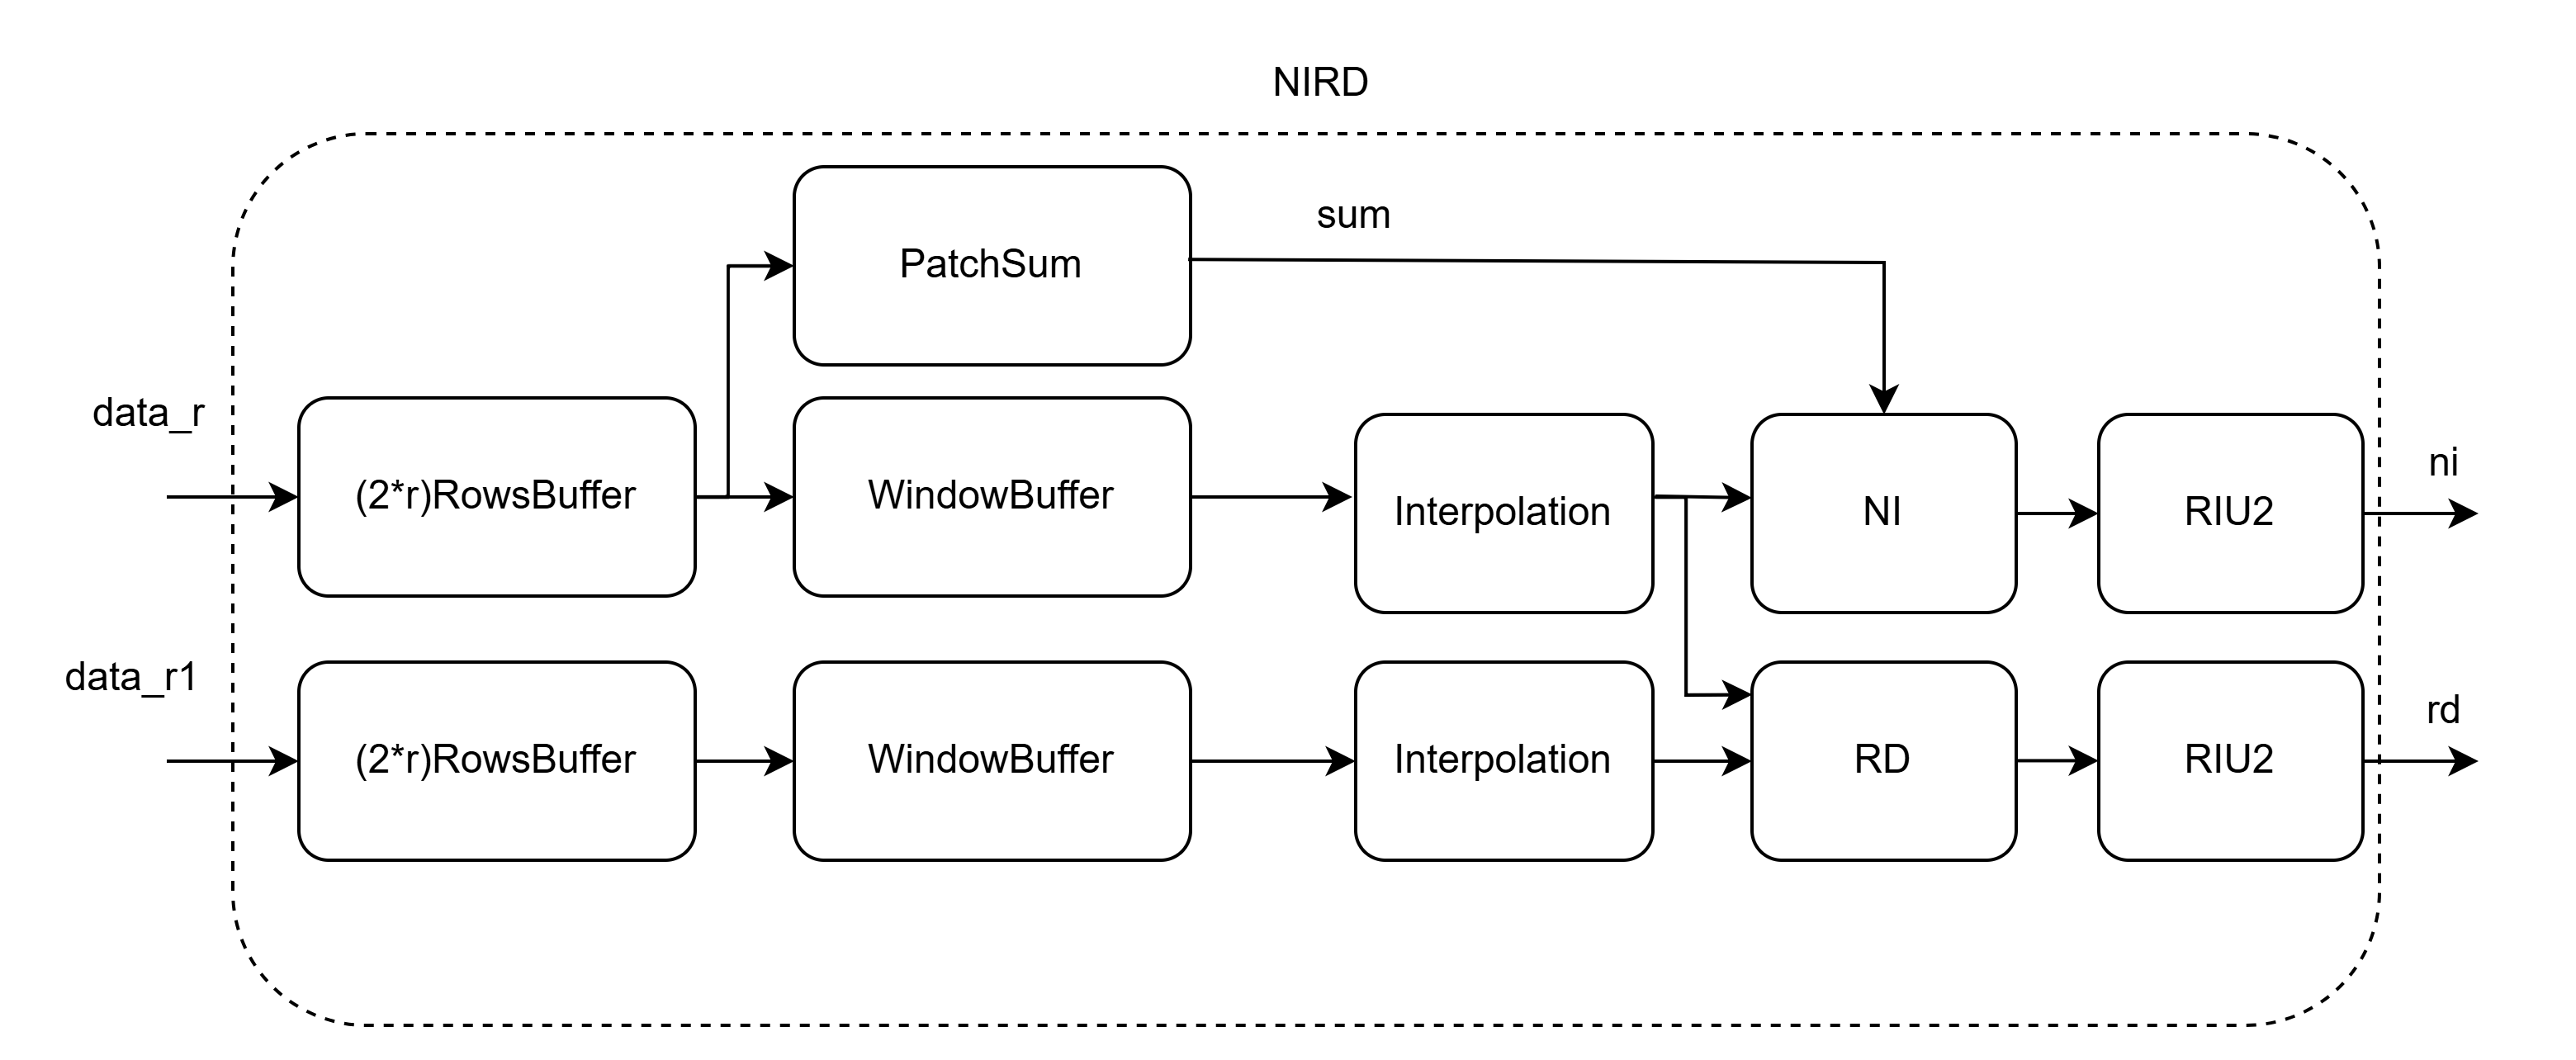
\includegraphics[width=\linewidth]{figures/nirdArch.png}
    \caption{Sơ đồ khối của mô-đun NIRD}
    \label{fig:nirdArch}
\end{figure}
\begin{figure}[!ht]
    \centering
    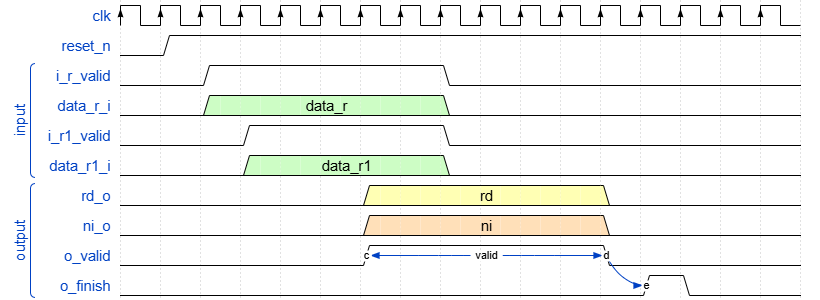
\includegraphics[width=\linewidth]{figures/nird.png}
    \caption{Dạng sóng của mô-đun NIRD}
    \label{fig:nird}
\end{figure}

\subsubsection{Đặc tả mô-đun Interpolation}
mô-đun này sẽ thực hiện chức năng tính toán giá trị chưa biết ở một vài vị trí bán kính bằng phương pháp nội suy. Vì phương pháp này sẽ xuất hiện các giá trị thập phân, để tiện cho việc biểu diễn, sinh viên sử dụng dấu phẩy tĩnh với 8-bit phần nguyên và 16-bit phần thập phân, tổng cộng là 24-bit cho dữ liệu đầu ra. Các dữ liệu ở các góc đặc biệt như 0, 90, 180, 270 độ sẽ không cần thực hiện nội suy, do đó, trong mô-đun cũng sẽ thực thi chức năng đệm dữ liệu để đảm bảo đầu ra có đủ 8 giá trị trên đường tròn bán kính r ở tại một thời điểm. Vì phương pháp nội sử dụng là tuyến tính, do đó cần 4 điểm xung quanh vị trí cần tính, nên ứng với các góc 45, 135, 225 và 315 thì sễ cần đầy đủ 4 giá trị đầu vào để tính toán.

\begin{table}[!ht]
    \centering
    \renewcommand{\arraystretch}{1.3} % Tăng khoảng cách dòng
        \caption{Tham số của mô-đun Interpolation}
    \begin{tabular}{|p{3cm} p{4cm} p{8cm}|}
        \hline
        \rowcolor{gray!30}
        \textbf{Tham số } & \textbf{Giá trị mặc định}  & \textbf{Mô tả} \\
        \hline
        R & 2 & Kích thước bán kính 
        \\ \hline
        ANGLE & 45 & Giá trị góc
        \\
        \hline
    \end{tabular}

    \label{tab:paramListInterpolation}
\end{table}
\begin{table}[H]
    \centering
    \renewcommand{\arraystretch}{1.2}
        \caption{Danh sách các tín hiệu của mô-đun Interpolation}
    \begin{tabular}{|p{3cm} p{2cm} p{2cm} p{8cm}|}
        \hline
        \rowcolor{gray!30}
        \textbf{Tên tín hiệu} & \textbf{Độ rộng} & \textbf{Vào ra} & \textbf{Mô tả} \\
        \hline
        clk & 1 & Vào & Tín hiệu clock \\
        \hline
        rst\_n & 1 & Vào & Tín hiệu reset đồng bộ, kích hoạt mức thấp \\
        \hline 
        i\_valid & 1 & Vào & Thông báo rằng dữ liệu đầu vào là hợp lệ \\
        \hline
        i\_finish & 1 & Vào & Thông báo không còn dữ liệu đầu vào \\
        \hline
        S\_0\_i & 8 & Vào & Dữ liệu đầu vào tại góc 0 độ \\
        \hline
        S\_90\_i & 8 & Vào & Dữ liệu đầu vào tại góc 90 độ \\
        \hline
        S\_180\_i & 8 & Vào & Dữ liệu đầu vào tại góc 180 độ \\
        \hline
        S\_270\_i & 8 & Vào & Dữ liệu đầu vào tại góc 270 độ \\
        \hline
        S\_45\_i\_1 & 8 & Vào & Dữ liệu đầu vào thứ 1 tại hướng 45 độ \\
        \hline
        S\_45\_i\_2 & 8 & Vào & Dữ liệu đầu vào thứ 2 tại hướng 45 độ \\
        \hline
        S\_45\_i\_3 & 8 & Vào & Dữ liệu đầu vào thứ 3 tại hướng 45 độ \\
        \hline
        S\_45\_i\_4 & 8 & Vào & Dữ liệu đầu vào thứ 4 tại hướng 45 độ \\
        \hline
        S\_135\_i\_1 & 8 & Vào & Dữ liệu đầu vào thứ 1 tại hướng 135 độ \\
        \hline
        S\_135\_i\_2 & 8 & Vào & Dữ liệu đầu vào thứ 2 tại hướng 135 độ \\
        \hline
        S\_135\_i\_3 & 8 & Vào & Dữ liệu đầu vào thứ 3 tại hướng 135 độ \\
        \hline
        S\_135\_i\_4 & 8 & Vào & Dữ liệu đầu vào thứ 4 tại hướng 135 độ \\
        \hline
        S\_225\_i\_1 & 8 & Vào & Dữ liệu đầu vào thứ 1 tại hướng 225 độ \\
        \hline
        S\_225\_i\_2 & 8 & Vào & Dữ liệu đầu vào thứ 2 tại hướng 225 độ \\
        \hline
        S\_225\_i\_3 & 8 & Vào & Dữ liệu đầu vào thứ 3 tại hướng 225 độ \\
        \hline
        S\_225\_i\_4 & 8 & Vào & Dữ liệu đầu vào thứ 4 tại hướng 225 độ \\
        \hline
        S\_315\_i\_1 & 8 & Vào & Dữ liệu đầu vào thứ 1 tại hướng 315 độ \\
        \hline
        S\_315\_i\_2 & 8 & Vào & Dữ liệu đầu vào thứ 2 tại hướng 315 độ \\
        \hline
        S\_315\_i\_3 & 8 & Vào & Dữ liệu đầu vào thứ 3 tại hướng 315 độ \\
        \hline
        S\_315\_i\_4 & 8 & Vào & Dữ liệu đầu vào thứ 4 tại hướng 315 độ \\
        \hline
        S1\_o --> S8\_o & 24 & Ra & Dữ liệu nội suy đầu ra hướng từ 0 -> 315 độ \\
        \hline
        o\_valid & 1 & Ra & Thông báo đầu ra là hợp lệ\\
        \hline
        o\_finish & 1 & Ra & Tín hiệu cho biết đã hết dữ liệu đầu ra \\
        \hline
    \end{tabular}

    \label{tab:signalListInterpolation}
\end{table}












\subsubsection{Đặc tả mô-đun NI}
mô-đun NI sẽ tính toán giá trị của 8 điểm trong đường tròn bán kính r, theo mô tả tại bảng \ref{tab:signalListNI} là từ S1\_r -> S8\_r với giá trị sum\_i. Theo công thức \ref{eq:relbp_ni} thì cần tính trung bình tổng của một cửa sổ, tuy nhiên thực hiện bộ chia sẽ tốn nhiều tài nguyên và phức tạp hơn bộ nhân, do đó mô-đun sẽ triển khai nhân các giá trị đầu vào với tham số \textbf{GAIN}.
\begin{table}[!ht]
    \centering
    \renewcommand{\arraystretch}{1.3} % Tăng khoảng cách dòng
        \caption{Tham số của mô-đun NI}
    \begin{tabular}{|p{3cm} p{4cm} p{8cm}|}
        \hline
        \rowcolor{gray!30}
        \textbf{Tham số } & \textbf{Giá trị mặc định}  & \textbf{Mô tả} \\
        \hline
        WIDTH & 10 & Độ rộng bit của dữ liệu đầu vào sum
        \\ \hline
        GAIN & 25 & Hệ số nhân đối với sum
        \\
        \hline
    \end{tabular}

    \label{tab:paramListNI}
\end{table}
\begin{table}[!ht]
    \centering
    \renewcommand{\arraystretch}{1.3} % Tăng khoảng cách dòng
        \caption{Danh sách các tín hiệu của mô-đun NI}
    \begin{tabular}{|p{3cm} p{2cm} p{2cm} p{8cm}|}
        \hline
        \rowcolor{gray!30}
        \textbf{Tên tín hiệu} & \textbf{Độ rộng} & \textbf{Vào/Ra} & \textbf{Mô tả} \\
        \hline
        clk & 1 & Vào & Tín hiệu clock \\
        \hline
        rst\_n & 1 & Vào & Tín hiệu reset đồng bộ, mức kích hoạt thấp \\
        \hline
        i\_valid & 1 & Vào & Tín hiệu báo dữ liệu đầu vào là hợp lệ \\
        \hline
        i\_finish & 1 & Vào & Tín hiệu báo đã hết dữ liệu đầu vào \\
        \hline
        S1\_r --> S8\_r & 24 & Vào & Các giá trị đầu vào từ 8 hướng tại bán kính r\\
        \hline
        sum\_i & WIDTH & Vào & Tổng giá trị từ mô-đun trước \\
        \hline
        o\_valid & 1 & Ra & Tín hiệu báo dữ liệu đầu ra là hợp lệ\\
        \hline
        o\_finish & 1 & Ra & Tín hiệu báo đã hết dữ liệu đầu ra \\
        \hline
        bit1\_o --> bit8\_o & 1 & Ra & 8 giá trị đầu ra nhị phân ứng với 8 hướng \\
        \hline
    \end{tabular}

    \label{tab:signalListNI}
\end{table}

\begin{figure}[H]
    \centering
    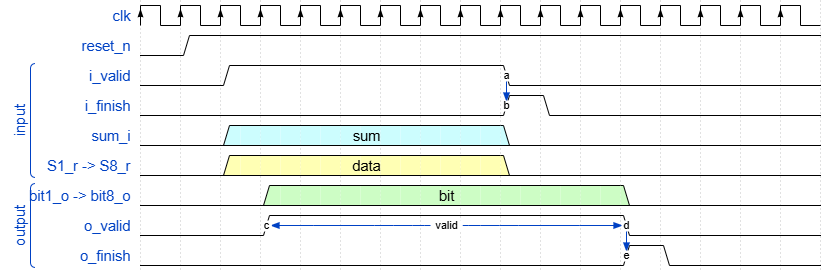
\includegraphics[width=\linewidth]{figures/ni.png}
    \caption{Dạng sóng của mô-đun NI}
    \label{fig:ni}
\end{figure}

\subsubsection{Đặc tả mô-đun RD}
mô-đun RD sẽ tính giá trị mô tả bằng cách so sánh lần lượt các giá trị nằm trên 2 đường tròn bán kính r và r1. Để thuận tiện cho việc đồng bộ dữ liệu, đầu vào sẽ cần có đủ 8 dữ liệu bán kính r và 8 dữ liệu bán kính r1. Dữ liệu đầu ra sẽ lần lượt là 8 bit lần lượt với từng vị trí trên đường tròn. Ví dụ tại vị trí 0 độ, sẽ so sánh giá trị S1\_r và S1\_r1, tương tự với các vị trí khác. 
\begin{table}[H]
    \centering
    \renewcommand{\arraystretch}{1.3} % Tăng khoảng cách dòng
        \caption{Danh sách các tín hiệu của mô-đun RD}
    \begin{tabular}{|p{3cm} p{2cm} p{2cm} p{8cm}|}
        \hline
        \rowcolor{gray!30}
        \textbf{Tên tín hiệu} & \textbf{Độ rộng} & \textbf{Vào/Ra} & \textbf{Mô tả} \\
        \hline
        clk & 1 & Vào & Tín hiệu clock \\
        \hline
        rst\_n & 1 & Vào & Tín hiệu reset đồng bộ, mức kích hoạt thấp \\
        \hline
        i\_valid & 1 & Vào & Tín hiệu báo dữ liệu đầu vào là hợp lệ \\
        \hline
        i\_finish & 1 & Vào & Tín hiệu báo đã hết dữ liệu đầu vào \\
        \hline
        S1\_r --> S8\_r & 24 & Vào & Các giá trị đầu vào từ 8 hướng tại bán kính r\\
        \hline
        S1\_r1 --> S8\_r1 & 24 & Vào & Các giá trị đầu vào từ 8 hướng tại bán kính r1\\
        \hline
        o\_valid & 1 & Ra & Tín hiệu báo dữ liệu đầu ra là hợp lệ\\
        \hline
        o\_finish & 1 & Ra & Tín hiệu báo đã hết dữ liệu đầu ra \\
        \hline
        bit1\_o --> bit8\_o & 1 & Ra & 8 giá trị đầu ra nhị phân ứng với 8 hướng \\
        \hline
    \end{tabular}

    \label{tab:signalListRD}
\end{table}
\begin{figure}[!ht]
    \centering
    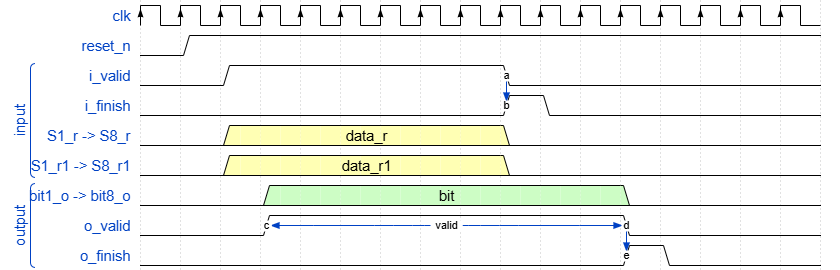
\includegraphics[width=\linewidth]{figures/rd.png}
    \caption{Dạng sóng của mô-đun RD}
    \label{fig:rd}
\end{figure}
\newpage
\subsubsection{Đặc tả mô-đun RIU2}
mô-đun RIU2 sẽ tính toán ra các đặc trưng dựa vào 8-bit đầu vào được tính hoặc từ mô-đun NI hoặc từ mô-đun RD theo công thức \ref{eq:riu2}.
\begin{table}[!ht]
    \centering
    \renewcommand{\arraystretch}{1.3} % Tăng khoảng cách dòng
        \caption{Danh sách các tín hiệu của mô-đun RIU2}
    \begin{tabular}{|p{3cm} p{2cm} p{2cm} p{8cm}|}
        \hline
        \rowcolor{gray!30}
        \textbf{Tên tín hiệu} & \textbf{Độ rộng} & \textbf{Vào/Ra} & \textbf{Mô tả} \\
        \hline
        clk & 1 & Vào & Tín hiệu clock \\
        \hline
        rst\_n & 1 & Vào & Tín hiệu reset đồng bộ, mức kích hoạt thấp \\
        \hline
        i\_valid & 1 & Vào & Tín hiệu báo dữ liệu đầu vào là hợp lệ \\
        \hline
        i\_finish & 1 & Vào & Tín hiệu báo đã hết dữ liệu đầu vào \\
        \hline
        bit1\_i --> bit8\_i & 1 & Vào & 8 giá trị nhị phân đầu vào\\
        \hline
        o\_valid & 1 & Ra & Tín hiệu báo dữ liệu đầu ra là hợp lệ\\
        \hline
        o\_finish & 1 & Ra & Tín hiệu báo đã hết dữ liệu đầu ra \\
        \hline
        data\_o & 4 & Ra & Giá trị riu2 \\
        \hline
    \end{tabular}

    \label{tab:signalListRIU2}
\end{table}
\begin{figure}[!ht]
    \centering
    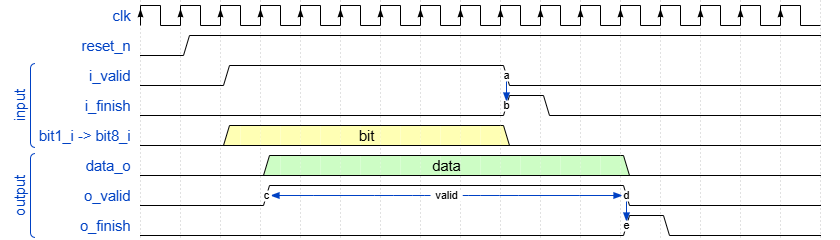
\includegraphics[width=\linewidth]{figures/riu2.png}
    \caption{Dạng sóng của mô-đun RIU2}
    \label{fig:riu2}
\end{figure}
\subsection{Đặc tả mô-đun JointHistogram}

\begin{figure}[H]
    \centering
    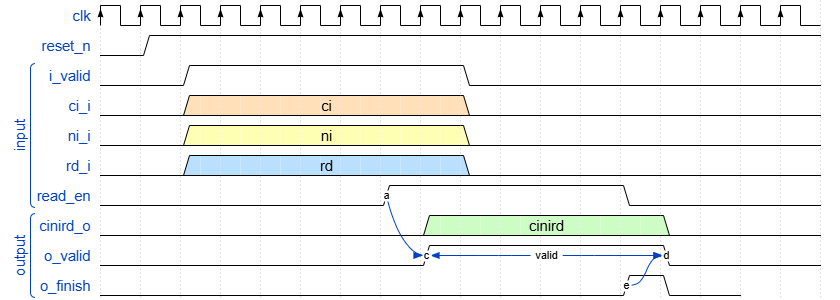
\includegraphics[width=\linewidth]{figures/jointHistogram.png}
    \caption{Biểu đồ sóng của mô-đun JointHistogram}
    \label{fig:jointHistogram}
\end{figure}
mô-đun JointHistogram sẽ có mục đích ghép 3 loại dữ liệu CI, NI và RD theo một công thức toán học nào đó để đạt được đặc trưng đầu ra. Công thức \ref{eq:joint} mô tả cách một đặc trưng được tính toán, mỗi lần đặc trưng này xuất hiện thì giá trị tại bộ nhớ nơi lưu trữ giá trị đấy được tăng lên 1 đơn vị. Vì ci chỉ nhận được giá trị từ 0 -> 1, các giá trị ni và rd sẽ chỉ nhận giá trị từ 0 -> 9 nên thực tế đặc trưng đầu ra có chiều dữ liệu là 200 ứng với mỗi r.
\begin{equation}
    f = ci*100 + ni*10 + rd
    \label{eq:joint}
\end{equation}
\begin{table}[!ht]
    \centering
    \renewcommand{\arraystretch}{1.3} % Tăng khoảng cách dòng
        \caption{Danh sách các tín hiệu của mô-đun JointHistogram}
    \begin{tabular}{|p{3cm} p{2cm} p{2cm} p{8cm}|}
        \hline
        \rowcolor{gray!30}
        \textbf{Tên tín hiệu} & \textbf{Độ rộng} & \textbf{Vào/Ra} & \textbf{Mô tả} \\
        \hline
        clk & 1 & Vào & Tín hiệu clock \\
        \hline
        rst\_n & 1 & Vào & Tín hiệu reset đồng bộ, mức kích hoạt thấp \\
        \hline
        i\_valid & 1 & Vào & Tín hiệu báo dữ liệu đầu vào là hợp lệ \\
        \hline
        ci\_i & 1 & Vào & Mô tả ci đầu vào
        \\ \hline
        ni\_i & 4 & Vào & Mô tả ni đầu vào
        \\ \hline
        rd\_i & 4 & Vào & Mô tả rd đầu vào
        \\ \hline
        read\_en & 1 & Vào & Tín hiệu cho phép đọc từ bộ nhớ
        \\ \hline
        cinird\_o & 16 & Ra & Đặc trưng đầu ra
        \\ \hline
        o\_valid & 1 & Ra & Thông báo dữ liệu đàu ra là hợp lệ
        \\ \hline
        o\_finish & 1 & Ra & Tín hiệu thông báo đã hết dữ liệu đầu ra
        \\
        \hline
    \end{tabular}

    \label{tab:signalListJointHistogram}
\end{table}